\title{Flatland\\ \large Fifth edition}
\author{\LARGE Edwin A. Abbott} 
\date{\today}
\documentclass[10pt, kindle, oneside]{kindle}
\usepackage[hmargin={5mm, 5mm}, vmargin={2mm, 5mm}]{geometry} 
\usepackage[english]{babel}
\usepackage[T1]{fontenc}
\usepackage{palatino}
\usepackage{graphicx} 
\usepackage[pdftex,
            pdfauthor={Edwin A. Abbott},
            pdftitle={Flatland},
            pdfsubject={},
            pdfkeywords={},
            pdfproducer={},
            pdfcreator={pdfTeX}]{hyperref}

%%%%%%%%%%%%%%%%%%%%%%%%%%%%%%%%%%%%%%%%%
%\overfullrule=1mm
%
\usepackage{microtype}
\setlength{\parindent}{5mm}
%
\tolerance=1
\emergencystretch=\maxdimen
\hyphenpenalty=10000
\hbadness=10000
%%%%%%%%%%%%%%%%%%%%%%%%%%%%%%%%%%%%%%%%%

\begin{document}
\maketitle
%%
\null\vfill
\begin{center}
    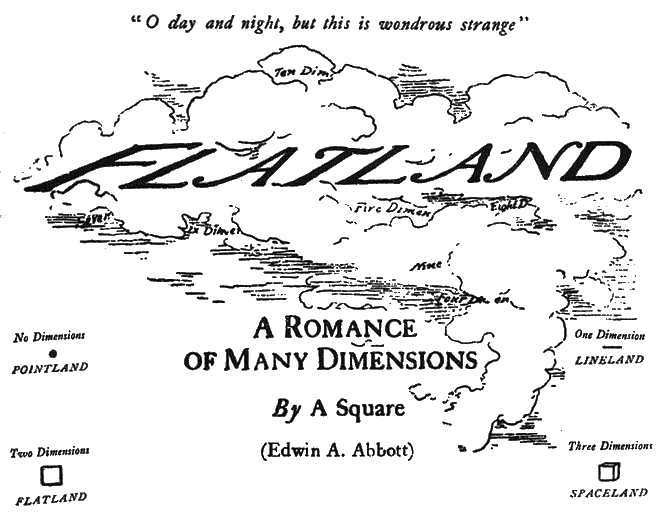
\includegraphics[trim=0mm 0mm 0mm 0mm,width=\linewidth]{flatland_cover}
\end{center}
\vfill\null
\clearpage
%%


\frontmatter
\chapter*{Dedication}


\footnotesize
\begin{center}
To\\
The Inhabitants of SPACE IN GENERAL\\
And H.C. IN PARTICULAR\\
This Work is Dedicated\\
By a Humble Native of Flatland\\
In the Hope that\\
Even as he was Initiated into the Mysteries\\
Of THREE DIMENSIONS\\
Having been previously conversant\\
With ONLY TWO\\
So the Citizens of that Celestial Region\\
May aspire yet higher and higher\\
To the Secrets of FOUR FIVE or EVEN SIX Dimensions\\
Thereby contributing\\
To the Enlargement of THE IMAGINATION\\
And the possible Development\\
Of that most rare and excellent Gift of MODESTY\\
Among the Superior Races\\
Of SOLID HUMANITY\\
\end{center}
\normalsize


\chapter*{Preface}


If my poor Flatland friend retained the vigour of mind which he enjoyed when
he began to compose these Memoirs, I should not now need to represent him in
this preface, in which he desires, fully, to return his thanks to his readers
and critics in Spaceland, whose appreciation has, with unexpected celerity,
required a second edition of this work; secondly, to apologize for certain
errors and misprints (for which, however, he is not entirely responsible);
and, thirdly, to explain on or two misconceptions. But he is not the Square he
once was. Years of imprisonment, and the still heavier burden of general
incredulity and mockery, have combined with the thoughts and notions, and much
also of the terminology, which he acquired during his short stay in Spaceland.
He has, therefore, requested me to reply in his behalf to two special
objections, one of an intellectual, the other of a moral nature.

The first objection is, that a Flatlander, seeing a Line, sees something that
must be thick to the eye as well as long to the eye (otherwise it would not be
visible, if it had not some thickness); and consequently he ought (it is
argued) to acknowledge that his countrymen are not only long and broad, but
also (though doubtless to a very slight degree) thick or high. This objection
is plausible, and, to Spacelanders, almost irresistible, so that, I confess,
when I first heard it, I knew not what to reply. But my poor old friend's
answer appears to me completely to meet it.

``I admit,'' said he --- when I mentioned to him this objection --- ``I admit the
truth of your critic's facts, but I deny his conclusions. It is true that we
have really in Flatland a Third unrecognized Dimension called `height,' just
as it also is true that you have really in Spaceland a Fourth unrecognized
Dimension, called by no name at present, but which I will call `extra-height.'
But we can no more take cognizance of our `height' than you can of your
`extra-height.' Even I --- who have been in Spaceland, and have had the
privilege of understanding for twenty-four hours the meaning of `height' ---
even I cannot now comprehend it, nor realize it by the sense of sight or by
any process of reason; I can but apprehend it by faith.''

``The reason is obvious. Dimension implied direction, implies measurement,
implies the more and the less. Now, all our lines are \emph{equally} and
\emph{infinitesimally} thick (or high, whichever you like); consequently, there is
nothing in them to lead our minds to the conception of that Dimension. No
`delicate micrometer' --- as has been suggested by one too hasty Spaceland
critic --- would in the least avail us; for we should not know \emph{what to measure,
nor in what direction}. When we see a Line, we see something that is long and
\emph{bright}; \emph{brightness}, as well as length, is necessary to the existence of a
Line; if the brightness vanishes, the Line is extinguished. Hence, all my
Flatland friends --- when I talk to them about the unrecognized Dimension which
is somehow visible in a Line --- say, `Ah, you mean \emph{brightness}': and when I
reply, `No, I mean a real Dimension,' they at once retort, `Then measure it,
or tell us in what direction it extends'; and this silences me, for I can do
neither. Only yesterday, when the Chief Circle (in other words our High
Priest) came to inspect the State Prison and paid me his seventh annual visit,
and when for the seventh time he put me the question, `Was I any better?' I
tried to prove to him that he was `high', as well as long and broad, although
he did not know it. But what was his reply? `You say I am ``high''; measure my
``high-ness'' and I will believe you.'. What could I do? How could I meet his
challenge? I was crushed; and he left the room triumphant.''

``Does this still seem strange to you? Then put yourself in a similar position.
Suppose a person of the Fourth Dimension, condescending to visit you, were to
say, `Whenever you open your eyes, you \emph{see} a Plane (which is of Two
Dimensions) and you \emph{infer} a Solid (which is of Three); but in reality you also
see (though you do not recognize) a Fourth Dimension, which is not colour nor
brightness nor anything of the kind, but a true Dimension, although I cannot
point out to you its direction, nor can you possibly measure it.' What would
you say to such a visitor? Would not you have him locked up? Well, that is my
fate: and it is as natural for us Flatlanders to lock up a Square for
preaching the Third Dimension, as it is for you Spacelanders to lock up a Cube
for preaching the Fourth. Alas, how strong a family likeness runs through
blind and persecuting humanity in all Dimensions! Points, Lines, Squares,
Cubes, Extra-Cubes --- we are all liable to the same errors, all alike the
Slavers of our respective Dimensional prejudices, as one of our Spaceland
poets has said --- `One touch of Nature makes all worlds akin.' ''~\footnote{The
Author desires me to add, that the misconceptions of some of his critics on
this matter has induced him to insert in his dialogue with
the Sphere, certain remarks which have a bearing on the point in question and
which he had previously omitted as being tedious and unnecessary.}

On this point the defence of the Square seems to me to be impregnable. I wish
I could say that his answer to the second (or moral) objection was equally
clear and cogent. It has been objected that he is a woman-hater; and as this
objection has been vehemently urged by those whom Nature's decree has
constituted the somewhat larger half of the Spaceland race, I should like to
remove it, so far as I can honestly do so. But the Square is so unaccustomed
to the use of the moral terminology of Spaceland that I should be doing him an
injustice if I were literally to transcribe his defence against this charge.
Acting, therefore, as his interpreter and summarizer, I gather that in the
course of an imprisonment of seven years he has himself modified his own
personal views, both as regards Women and as regards the Isosceles or Lower
Classes. Personally, he now inclines to the opinion of the Sphere  that the
Straight Lines are in many important respects superior to the
Circles. But, writing as a Historian, he has identified himself (perhaps too
closely) with the views generally adopted by Flatland, and (as he has been
informed) even by Spaceland, Historians; in whose pages (until very recent
times) the destinies of Women and of the masses of mankind have seldom been
deemed worthy of mention and never of careful consideration.

In a still more obscure passage he now desires to disavow the Circular or
aristocratic tendencies with which some critics have naturally credited him.
While doing justice to the intellectual power with which a few Circles have
for many generations maintained their supremacy over immense multitudes of
their countrymen, he believes that the facts of Flatland, speaking for
themselves without comment on his part, declare that Revolutions cannot always
be suppressed by slaughter, and that Nature, in sentencing the Circles to
infecundity, has condemned them to ultimate failure --- ``and herein,'' he says,
``I see a fulfillment of the great Law of all worlds, that while the wisdom of
Man thinks it is working one thing, the wisdom of Nature constrains it to work
another, and quite a different and far better thing.'' For the rest, he begs
his readers not to suppose that every minute detail in the daily life of
Flatland must needs correspond to some other detail in Spaceland; and yet he
hopes that, taken as a whole, his work may prove suggestive as well as
amusing, to those Spacelanders of moderate and modest minds who --- speaking of
that which is of the highest importance, but lies beyond experience --- decline
to say on the one hand, ``This can never be,'' and on the other hand, ``It must
needs be precisely thus, and we know all about it.''


\mainmatter
\part{This World}
\chapter{Of the Nature of Flatland} 


I call our world Flatland, not because we
call it so, but to make its nature clearer to you, my happy readers, who are
privileged to live in Space.

Imagine a vast sheet of paper on which straight Lines, Triangles, Squares,
Pentagons, Hexagons, and other figures, instead of remaining fixed in their
places, move freely about, on or in the surface, but without the power of
rising above or sinking below it, very much like shadows --- only hard with
luminous edges --- and you will then have a pretty correct notion of my country
and countrymen. Alas, a few years ago, I should have said ``my universe'': but
now my mind has been opened to higher views of things.

In such a country, you will perceive at once that it is impossible that there
should be anything of what you call a ``solid'' kind; but I dare say you will
suppose that we could at least distinguish by sight the Triangles, Squares,
and other figures, moving about as I have described them. On the contrary, we
could see nothing of the kind, not at least so as to distinguish one figure
from another. Nothing was visible, nor could be visible, to us, except
Straight Lines; and the necessity of this I will speedily demonstrate.

Place a penny on the middle of one of your tables in Space; and leaning over
it, look down upon it. It will appear a circle.

But now, drawling back to the edge of the table, gradually lower your eye
(thus bringing yourself more and more into the condition of the inhabitants of
Flatland), and you will find the penny becoming more and more oval to your
view, and at last when you have placed your eye exactly on the edge of the
table (so that you are, as it were, actually a Flatlander) the penny will then
have ceased to appear oval at all, and will have become, so far as you can
see, a straight line.

The same thing would happen if you were to treat in the same way a Triangle,
or a Square, or any other figure cut out of pasteboard. As soon as you look at
it with your eye on the edge of the table, you will find that it ceases to
appear to you as a figure, and that it becomes in appearance a straight line.
Take for example an equilateral Triangle --- who represents with us a Tradesman
of the respectable class. Figure 1 represents the Tradesman as you would see
him while you were bending over him from above; figures 2 and 3 represent the
Tradesman, as you would see him if your eye were close to the level, or all
but on the level of the table; and if your eye were quite on the level of the
table (and that is how we see him in Flatland) you would see nothing but a
straight line.

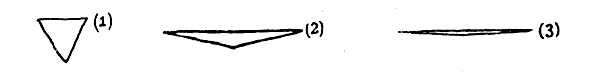
\includegraphics[trim=0mm 0mm 0mm 0mm,width=\linewidth]{fig1}

When I was in Spaceland I heard that your sailors have very similar
experiences while they traverse your seas and discern some distant island or
coast lying on the horizon. The far-off land may have bays, forelands, angles
in and out to any number and extent; yet at a distance you see none of these
(unless indeed your sun shines bright upon them revealing the projections and
retirements by means of light and shade), nothing but a grey unbroken line
upon the water.

Well, that is just what we see when one of our triangular or other
acquaintances comes towards us in Flatland. As there is neither sun with us,
nor any light of such a kind as to make shadows, we have none of the helps to
the sight that you have in Spaceland. If our friend comes closer to us we see
his line becomes larger; if he leaves us it becomes smaller; but still he
looks like a straight line; be he a Triangle, Square, Pentagon, Hexagon,
Circle, what you will --- a straight Line he looks and nothing else.

You may perhaps ask how under these disadvantageous circumstances we are able
to distinguish our friends from one another: but the answer to this very
natural question will be more fitly and easily given when I come to describe
the inhabitants of Flatland. For the present let me defer this subject, and
say a word or two about the climate and houses in our country.


\chapter{Of the Climate and Houses in Flatland}


As with you, so also with us, there are four points of the compass North,
South, East, and West.

There being no sun nor other heavenly bodies,
it is impossible for us to determine the North in the usual way; but we have a
method of our own. By a Law of Nature with us, there is a constant attraction
to the South; and, although in temperate climates this is very slight --- so
that even a Woman in reasonable health can journey several furlongs northward
without much difficulty --- yet the hampering effect of the southward attraction
is quite sufficient to serve as a compass in most parts of our earth.
Moreover, the rain (which falls at stated intervals) coming always from the
North, is an additional assistance; and in the towns we have the guidance of
the houses, which of course have their side-walls running for the most part
North and South, so that the roofs may keep off the rain from the North. In
the country, where there are no houses, the trunks of the trees serve as some
sort of guide. Altogether, we have not so much difficulty as might be expected
in determining our bearings.

Yet in our more temperate regions, in which the southward attraction is hardly
felt, walking sometimes in a perfectly desolate plain where there have been no
houses nor trees to guide me, I have been occasionally compelled to remain
stationary for hours together, waiting till the rain came before continuing my
journey. On the weak and aged, and especially on delicate Females, the force
of attraction tells much more heavily than on the robust of the Male Sex, so
that it is a point of breeding, if you meet a Lady in the street, always to
give her the North side of the way --- by no means an easy thing to do always at
short notice when you are in rude health and in a climate where it is
difficult to tell your North from your South.

Windows there are none in our houses: for the light comes to us alike in our
homes and out of them, by day and by night, equally at all times and in all
places, whence we know not. It was in old days, with our learned men, an
interesting and oft-investigate question, ``What is the origin of light?'' and
the solution of it has been repeatedly attempted, with no other result than to
crowd our lunatic asylums with the would-be solvers. Hence, after fruitless
attempts to suppress such investigations indirectly by making them liable to a
heavy tax, the Legislature, in comparatively recent times, absolutely
prohibited them. I --- alas, I alone in Flatland --- know now only too well the
true solution of this mysterious problem; but my knowledge cannot be made
intelligible to a single one of my countrymen; and I am mocked at --- I, the
sole possessor of the truths of Space and of the theory of the introduction of
Light from the world of three Dimensions --- as if I were the maddest of the
mad! But a truce to these painful digressions: let me return to our homes.

The most common form for the construction of a house is five-sided or
pentagonal, as in the annexed figure. The two Northern sides RO, OF,
constitute the roof, and for the most part have no doors; on the East is a
small door for the Women; on the West a much larger one for the Men; the South
side or floor is usually doorless.
\begin{center}
    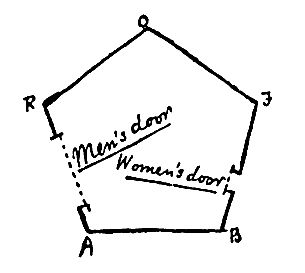
\includegraphics[trim=0mm 0mm 0mm 0mm, scale=0.5]{fig2}
\end{center}

Square and triangular houses are not allowed, and for this reason. The angles
of a Square (and still more those of an equilateral Triangle,) being much more
pointed than those of a Pentagon, and the lines of inanimate objects (such as
houses) being dimmer than the lines of Men and Women, it follows that there is
no little danger lest the points of a square of triangular house residence
might do serious injury to an inconsiderate or perhaps absentminded traveller
suddenly running against them: and therefore, as early as the eleventh century
of our era, triangular houses were universally forbidden by Law, the only
exceptions being fortifications, powder-magazines, barracks, and other state
buildings, which is not desirable that the general public should approach
without circumspection.

At this period, square houses were still everywhere permitted, though
discouraged by a special tax. But, about three centuries afterwards, the Law
decided that in all towns containing a population above ten thousand, the
angle of a Pentagon was the smallest house-angle that could be allowed
consistently with the public safety. The good sense of the community has
seconded the efforts of the Legislature; and now, even in the country, the
pentagonal construction has superseded every other. It is only now and then in
some very remote and backward agricultural district that an antiquarian may
still discover a square house.


\chapter{Concerning the Inhabitants of Flatland}


The greatest length or breadth of a full grown inhabitant of Flatland may be
estimated at about eleven of your inches. Twelve inches may be regarded as a
maximum.

Our Women are Straight Lines.

Our Soldiers and Lowest Class of Workmen are Triangles with two equal sides,
each about eleven inches long, and a base or third side so short (often not
exceeding half an inch) that they form at their vertices a very sharp and
formidable angle. Indeed when their bases are of the most degraded type (not
more than the eighth part of an inch in size), they can hardly be
distinguished from Straight lines or Women; so extremely pointed are their
vertices. With us, as with you, these Triangles are distinguished from others
by being called Isosceles; and by this name I shall refer to them in the
following pages.

Our Middle Class consists of Equilateral or Equal-Sided Triangles.

Our Professional Men and Gentlemen are Squares (to which class I myself
belong) and Five-Sided Figures or Pentagons.

Next above these come the Nobility, of whom there are several degrees,
beginning at Six-Sided Figures, or Hexagons, and from thence rising in the
number of their sides till they receive the honourable title of Polygonal, or
many-Sided. Finally when the number of the sides becomes so numerous, and the
sides themselves so small, that the figure cannot be distinguished from a
circle, he is included in the Circular or Priestly order; and this is the
highest class of all.

It is a Law of Nature with us that a male child shall have one more side than
his father, so that each generation shall rise (as a rule) one step in the
scale of development and nobility. Thus the son of a Square is a Pentagon; the
son of a Pentagon, a Hexagon; and so on.

But this rule applies not always to the Tradesman, and still less often to the
Soldiers, and to the Workmen; who indeed can hardly be said to deserve the
name of human Figures, since they have not all their sides equal. With them
therefore the Law of Nature does not hold; and the son of an Isosceles (\emph{i.e.} a
Triangle with two sides equal) remains Isosceles still. Nevertheless, all hope
is not shut out, even from the Isosceles, that his posterity may ultimately
rise above his degraded condition. For, after a long series of military
successes, or diligent and skillful labours, it is generally found that the
more intelligent among the Artisan and Soldier classes manifest a slight
increase of their third side or base, and a shrinkage of the two other sides.
Intermarriages (arranged by the Priests) between the sons and daughters of
these more intellectual members of the lower classes generally result in an
offspring approximating still more to the type of the Equal-Sided Triangle.

Rarely --- in proportion to the vast numbers of Isosceles births --- is a genuine
and certifiable Equal-Sided Triangle produced from Isosceles 
parents~\footnote{``What need of a certificate?'' a Spaceland critic may ask: ``Is not
the procreation of a Square Son a certificate from Nature herself, proving the
Equal-sidedness of the Father?'' I reply that no Lady of any position will
marry an uncertified Triangle. Square offspring has sometimes resulted from a
slightly Irregular Triangle; but in almost every such case the Irregularity of
the first generation is visited on the third; which either fails to attain the
Pentagonal rank, or relapses to the Triangular.}. Such a birth requires, as
its antecedents, not only a series of carefully arranged intermarriages, but
also a long-continued exercise of frugality and self-control on the part of
the would-be ancestors of the coming Equilateral, and a patient, systematic,
and continuous development of the Isosceles intellect through many
generations.

The birth of a True Equilateral Triangle from Isosceles parents is the subject
of rejoicing in our country for many furlongs around. After a strict
examination conducted by the Sanitary and Social Board, the infant, if
certified as Regular, is with solemn ceremonial admitted into the class of
Equilaterals. He is then immediately taken from his proud yet sorrowing
parents and adopted by some childless Equilateral, who is bound by oath never
to permit the child henceforth to enter his former home or so much as to look
upon his relations again, for fear lest the freshly developed organism may, by
force of unconscious imitation, fall back again into his hereditary level.

The occasional emergence of an Equilateral from the ranks of his serf-born
ancestors is welcomed, not only by the poor serfs themselves, as a gleam of
light and hope shed upon the monotonous squalor of their existence, but also
by the Aristocracy at large; for all the higher classes are well aware that
these rare phenomena, while they do little or nothing to vulgarize their own
privileges, serve as almost useful barrier against revolution from below.

Had the acute-angled rabble been all, without exception, absolutely destitute
of hope and of ambition, they might have found leaders in some of their many
seditious outbreaks, so able as to render their superior numbers and strength
too much even for the wisdom of the Circles. But a wise ordinance of Nature
has decreed that, in proportion as the working-classes increase in
intelligence, knowledge, and all virtue, in that same proportion their acute
angle (which makes them physically terrible) shall increase also and
approximate to their comparatively harmless angle of the Equilateral Triangle.
Thus, in the most brutal and formidable off the soldier class --- creatures
almost on a level with women in their lack of intelligence --- it is found that,
as they wax in the mental ability necessary to employ their tremendous
penetrating power to advantage, so do they wane in the power of penetration
itself.

How admirable is this Law of Compensation! And how perfect a proof of the
natural fitness and, I may almost say, the divine origin of the aristocratic
constitution of the States of Flatland! By a judicious use of this Law of
Nature, the Polygons and Circles are almost always able to stifle sedition in
its very cradle, taking advantage of the irrepressible and boundless
hopefulness of the human mind. Art also comes to the aid of Law and Order. It
is generally found possible --- by a little artificial compression or expansion
on the part of the State physicians --- to make some of the more intelligent
leaders of a rebellion perfectly Regular, and to admit them at once into the
privileged classes; a much larger number, who are still below the standard,
allured by the prospect of being ultimately ennobled, are induced to enter the
State Hospitals, where they are kept in honourable confinement for life; one
or two alone of the most obstinate, foolish, and hopelessly irregular are led
to execution.

Then the wretched rabble of the Isosceles, planless and leaderless, are ether
transfixed without resistance by the small body of their brethren whom the
Chief Circle keeps in pay for emergencies of this kind; or else more often, by
means of jealousies and suspicious skillfully fomented among them by the
Circular party, they are stirred to mutual warfare, and perish by one
another's angles. No less than one hundred and twenty rebellions are recorded
in our annals, besides minor outbreaks numbered at two hundred and
thirty-five; and they have all ended thus.


\chapter{Concerning the Women}


If our highly pointed Triangles of the Soldier class are formidable, it may be
readily inferred that far more formidable are our Women. For, if a Soldier is
a wedge, a Woman is a needle; being, so to speak, \emph{all} point, at least at the
two extremities. Add to this the power of making herself practically invisible
at will, and you will perceive that a Female, in Flatland, is a creature by no
means to be trifled with.

But here, perhaps, some of my younger Readers may ask \emph{how} a woman in Flatland
can make herself invisible. This ought, I think, to be apparent without any
explanation. However, a few words will make it clear to the most unreflecting.

Place a needle on the table. Then, with your eye on the level of the table,
look at it side-ways, and you see the whole length of it; but look at it
end-ways, and you see nothing but a point, it has become practically
invisible. Just so is it with one of our Women. When her side is turned
towards us, we see her as a straight line; when the end containing her eye or
mouth --- for with us these two organs are identical --- is the part that meets
our eye, then we see nothing but a highly lustrous point; but when the back is
presented to our view, then --- being only sub-lustrous, and, indeed, almost as
dim as an inanimate object --- her hinder extremity serves her as a kind of
Invisible Cap.

The dangers to which we are exposed from our Women must now be manifest to the
meanest capacity in Spaceland. If even the angle of a respectable Triangle in
the middle class is not without its dangers; if to run against a Working Man
involves a gash; if collision with an Officer of the military class
necessitates a serious wound; if a mere touch from the vertex of a Private
Soldier brings with it danger of death; --- what can it be to run against a
woman, except absolute and immediate destruction? And when a Woman is
invisible, or visible only as a dim sub-lustrous point, how difficult must it
be, even for the most cautious, always to avoid collision!

Many are the enactments made at different times in the different States of
Flatland, in order to minimize this peril; and in the Southern and less
temperate climates, where the force of gravitation is greater, and human
beings more liable to casual and involuntary motions, the Laws concerning
Women are naturally much more stringent. But a general view of the Code may be
obtained from the following summary: ---

Every house shall have one entrance on the Eastern side, for the use of
Females only; by which all females shall enter ``in a becoming and respectful
manner''~\footnote{When I was in Spaceland I understood that some of your
Priestly circles have in the same way a separate entrance for Villagers,
Farmers and Teachers of Board Schools (\emph{Spectator}, Sept. 1884, P. 1255) that
they may ``approach in a becoming and respectful manner.''} and not by the Men's
or Western door.  No Female shall walk in any public place without continually
keeping up her Peace-cry, under penalty of death.  Any Female, duly certified
to be suffering from St. Vitus's Dance, fits, chronic cold accompanied by
violent sneezing, or any disease necessitating involuntary motions, shall be
instantly destroyed.  In some of the States there is an additional Law
forbidding Females, under penalty of death, from walking or standing in any
public place without moving their backs constantly from right to left so as to
indicate their presence to those behind them; others oblige a Woman, when
travelling, to be followed by one of her sons, or servants, or by her husband;
others confine Women altogether to their houses except during the religious
festivals. But it has been found by the wisest of our Circles or Statesmen
that the multiplication of restrictions on Females tends not only to the
debilitation and diminution of the race, but also to the increase of domestic
murders to such an extent that a State loses more than it gains by a too
prohibitive Code.

For whenever the temper of the Women is thus exasperated by confinement at
home or hampering regulations abroad, they are apt to vent their spleen upon
their husbands and children; and in the less temperate climates the whole male
population of a village has been sometimes destroyed in one or two hours of
simultaneous female outbreak. Hence the Three Laws, mentioned above, suffice
for the better regulated States, and may be accepted as a rough
exemplification of our Female Code.

After all, our principal safeguard is found, not in Legislature, but in the
interests of the Women themselves. For, although they can inflict
instantaneous death by a retrograde movement, yet unless they can at once
disengage their stinging extremity from the struggling body of their victim,
their own frail bodies are liable to be shattered.

The power of Fashion is also on our side. I pointed
out that in some less civilized States no female is suffered to stand in any
public place without swaying her back from right to left. This practice has
been universal among ladies of any pretensions to breeding in all
well-governed States, as far back as the memory of Figures can reach. It is
considered a disgrace to any state that legislation should have to enforce
what ought to be, and is in every respectable female, a natural instinct. The
rhythmical and, if I may so say, well-modulated undulation of the back in our
ladies of Circular rank is envied and imitated by the wife of a common
Equilateral, who can achieve nothing beyond a mere monotonous swing, like the
ticking of a pendulum; and the regular tick of the Equilateral is no less
admired and copied by the wife of the progressive and aspiring Isosceles, in
the females of whose family no ``back-motion'' of any kind has become as yet a
necessity of life. Hence, in every family of position and consideration, ``back
motion'' is as prevalent as time itself; and the husbands and sons in these
households enjoy immunity at least from invisible attacks.

Not that it must be for a moment supposed that our Women are destitute of
affection. But unfortunately the passion of the moment predominates, in the
Frail Sex, over every other consideration. This is, of course, a necessity
arising from their unfortunate conformation. For as they have no pretensions
to an angle, being inferior in this respect to the very lowest of the
Isosceles, they are consequently wholly devoid of brainpower, and have neither
reflection, judgment nor forethought, and hardly any memory. Hence, in their
fits of fury, they remember no claims and recognize no distinctions. I have
actually known a case where a Woman has exterminated her whole household, and
half an hour afterwards, when her rage was over and the fragments swept away,
has asked what has become of her husband and her children.

Obviously then a Woman is not to be irritated as long as she is in a position
where she can turn round. When you have them in their apartments --- which are
constructed with a view to denying them that power --- you can say and do what
you like; for they are then wholly impotent for mischief, and will not
remember a few minutes hence the incident for which they may be at this moment
threatening you with death, nor the promises which you may have found it
necessary to make in order to pacify their fury.

On the whole we got on pretty smoothly in our domestic
relations, except in the lower strata of the Military Classes. There the want
of tact and discretion on the part of the husbands produces at times
indescribable disasters. Relying too much on the offensive weapons of their
acute angles instead of the defensive organs of good sense and seasonable
simulations, these reckless creatures too often neglect the prescribed
construction of the women's apartments, or irritate their wives by ill-advised
expressions out of doors, which they refuse immediately to retract. Moreover a
blunt and stolid regard for literal truth indisposes them to make those lavish
promises by which the more judicious Circle can in a moment pacify his
consort. The result is massacre; not, however, without its advantages, as it
eliminates the more brutal and troublesome of the Isosceles; and by many of
our Circles the destructiveness of the Thinner Sex is regarded as one among
many providential arrangements for suppressing redundant population, and
nipping Revolution in the bud.

Yet even in our best regulated and most approximately Circular families I
cannot say that the ideal of family life is so high as with you in Spaceland.
There is peace, in so far as the absence of slaughter may be called by that
name, but there is necessarily little harmony of tastes or pursuits; and the
cautious wisdom of the Circles has ensured safety at the cost of domestic
comfort. In every Circular or Polygonal household it has been a habit from
time immemorial --- and now has become a kind of instinct among the women of our
higher classes --- that the mothers and daughters should constantly keep their
eyes and mouths towards their husband and his male friends; and for a lady in
a family of distinction to turn her back upon her husband would be regarded as
a kind of portent, involving loss of \emph{status}. But, as I shall soon shew, this
custom, though it has the advantage of safety, is not without disadvantages.

Moving with ease and smoothness in uttering words; of rapid speech;
nimble in speaking; glib; as, a flippant, voluble, tongue.  In the house of
the Working Man or respectable Tradesman --- where the wife is allowed to turn
her back upon her husband, while pursuing her household avocations --- there are
at least intervals of quiet, when the wife is neither seen nor heard, except
for the humming sound of the continuous Peace-cry; but in the homes of the
upper classes there is too often no peace. There the voluble mouth and bright
penetrating eye are ever directed toward the Master of the household; and
light itself is not more persistent than the stream of Feminine discourse. The
tact and skill which suffice to avert a Woman's sting are unequal to the task
of stopping a Woman's mouth; and as the wife has absolutely nothing to say,
and absolutely no constraint of wit, sense, or conscience to prevent her from
saying it, not a few cynics have been found to aver that they prefer the
danger of the death-dealing but inaudible sting to the safe sonorousness of a
Woman's other end.

To my readers in Spaceland the condition of our Women may seen truly
deplorable, and so indeed it is. A Male of the lowest type of the Isosceles
may look forward to some improvement of his angle, and to the ultimate
elevation of the whole of his degraded caste; but no Woman can entertain such
hopes for her sex. ``Once a Woman, always a Woman'' is a Decree of Nature; and
the very Laws of Evolution seem suspended in her disfavour. Yet at least we
can admire the wise Prearrangement which has ordained that, as they have no
hopes, so they shall have no memory to recall, and no forethought to
anticipate, the miseries and humiliations which are at once a necessity of
their existence and the basis of the constitution of Flatland.


\chapter{Of our Methods of Recognizing one another}


You, who are blessed with
shade as well as light, you, who are gifted with two eyes, endowed with a
knowledge of perspective, and charmed with the enjoyment of various colours,
you, who can actually see an angle, and contemplate the complete circumference
of a Circle in the happy region of the Three Dimensions --- how shall I make it
clear to you the extreme difficulty which we in Flatland experience in
recognizing one another's configuration?

Recall what I told you above. All beings in Flatland, animate and inanimate,
no matter what their form, present \emph{to our view} the same, or nearly the same,
appearance, viz.\@ that of a straight Line. How then can one be distinguished
from another, where all appear the same?

The answer is threefold. The first means of recognition is the sense of
hearing; which with us is far more highly developed than with you, and which
enables us not only to distinguish by the voice our personal friends, but even
to discriminate between different classes, at least so far as concerns the
three lowest orders, the Equilateral, the Square, and the Pentagon --- for the
Isosceles I take no account. But as we ascend the social scale, the process of
discriminating and being discriminated by hearing increases in difficulty,
partly because voices are assimilated, partly because the faculty of
voice-discrimination is a plebeian virtue not much developed among the
Aristocracy. And wherever there is any danger of imposture we cannot trust to
this method. Amongst our lowest orders, the vocal organs are developed to a
degree more than correspondent with those of hearing, so that an Isosceles can
easily feign the voice of a Polygon, and, with some training, that of a Circle
himself. A second method is therefore more commonly resorted to.

\emph{Feeling} is, among our Women and lower classes --- about our upper classes I
shall speak presently --- the principal test of recognition, at all events
between strangers, and when the question is, not as to the individual, but as
to the class. What therefore ``introduction'' is among the higher classes in
Spaceland, that the process of ``feeling'' is with us. ``Permit me to ask you to
feel and be felt by my friend Mr. So-and-so'' --- is still, among the more
old-fashioned of our country gentlemen in districts remote from towns, the
customary formula for a Flatland introduction. But in the towns, and among men
of business, the words ``be felt by'' are omitted and the sentence is
abbreviated to, ``Let me ask you to feel Mr. So-and-so''; although it is
assumed, of course, that the ``feeling'' is to be reciprocal. Among our still
more modern and dashing young gentlemen --- who are extremely averse to
superfluous effort and supremely indifferent to the purity of their native
language --- the formula is still further curtailed by the use of ``to feel'' in a
technical sense, meaning, ``to
recommend-for-the-purposes-of-feeling-and-being-felt''; and at this moment the
``slang'' of polite or fast society in the upper classes sanctions such a
barbarism as ``Mr. Smith, permit me to feel Mr. Jones.''.

Let not my Reader however suppose that ``feeling'' is with us the tedious
process that it would be with you, or that we find it necessary to feel right
round all the sides of every individual before we determine the class to which
he belongs. Long practice and training, begun in the schools and continued in
the experience of daily life, enable us to discriminate at once by the sense
of touch, between the angles of an equal-sided Triangle, Square, and Pentagon;
and I need not say that the brainless vertex of an acute-angled Isosceles is
obvious to the dullest touch. It is therefore not necessary, as a rule, to do
more than feel a single angle of an individual; and this, once ascertained,
tells us the class of the person whom we are addressing, unless indeed he
belongs to the higher sections of the nobility. There the difficulty is much
greater. Even a Master of Arts in our University of Wentbridge has been known
to confuse a ten-sided with a twelve-sided Polygon; and there is hardly a
Doctor of Science in or out of that famous University who could pretend to
decide promptly and unhesitatingly between a twenty-sided and a twenty-four
sided member of the Aristocracy.

Those of my readers who recall the extracts I gave above from the Legislative
code concerning Women, will readily perceive that the process of introduction
by contact requires some care and discretion. Otherwise the angles might
inflict on the unwary Feeler irreparable injury. It is essential for the
safety of the Feeler that the Felt should stand perfectly still. A start, a
fidgety shifting of the position, yes, even a violent sneeze, has been known
before now to prove fatal to the incautious, and to nip in the bud many a
promising friendship. Especially is this true among the lower classes of the
Triangles. With them, the eye is situated so far from their vertex that they
can scarcely take cognizance of what goes on at that extremity of their frame.
They are, moreover, of a rough coarse nature, not sensitive to the delicate
touch of the highly organized Polygon. What wonder then if an involuntary toss
of the head has ere now deprived the State of a valuable life!

I have heard that my excellent Grandfather --- one of the least irregular of his
unhappy Isosceles class, who indeed obtained, shortly before his decease, four
out of seven votes from the Sanitary and Social Board for passing him into the
class of the Equal-sided --- often deplored, with a tear in his venerable eye, a
miscarriage of this kind, which had occurred to his
great-great-great-Grandfather, a respectable Working Man with an angle or
brain of 59 degrees 30 minutes. According to his account, my unfortunate
Ancestor, being afflicted with rheumatism, and in the act of being felt by a
Polygon, by one sudden start accidentally transfixed the Great Man through the
diagonal and thereby, partly in consequence of his long imprisonment and
degradation, and partly because of the moral shock which pervaded the whole of
my Ancestor's relations, threw back our family a degree and a half in their
ascent towards better things. The result was that in the next generation the
family brain was registered at only 58 degrees, and not till the lapse of five
generations was the lost ground recovered, the full 60 degrees attained, and
the Ascent from the Isosceles finally achieved. And all this series of
calamities from one little accident in the process of Feeling.

At this point I think I hear some of my better educated readers exclaim, ``How
could you in Flatland know anything about angles and degrees, or minutes? We can
\emph{see} an angle, because we, in the region of Space, can see two straight lines
inclined to one another; but you, who can see nothing but on straight line at
a time, or at all events only a number of bits of straight lines all in one
straight line, --- how can you ever discern any angle, and much less register
angles of different sizes?''.

I answer that though we cannot \emph{see} angles, we can \emph{infer} them, and this with
great precision. Our sense of touch, stimulated by necessity, and developed by
long training, enables us to distinguish angles far more accurately than your
sense of sight, when unaided by a rule or measure of angles. Nor must I omit
to explain that we have great natural helps. It is with us a Law of Nature
that the brain of the Isosceles class shall begin at half a degree, or thirty
minutes, and shall increase (if it increases at all) by half a degree in every
generation until the goal of 60 degrees is reached, when the condition of
serfdom is quitted, and the freeman enters the class of Regulars.

Consequently, Nature herself supplies us with an ascending scale or Alphabet
of angles for half a degree up to 60 degrees, Specimen of which are placed in
every Elementary School throughout the land. Owing to occasional
retrogressions, to still more frequent moral and intellectual stagnation, and
to the extraordinary fecundity of the Criminal and Vagabond classes, there is
always a vast superfluity of individuals of the half degree and single degree
class, and a fair abundance of Specimens up to 10 degrees. These are
absolutely destitute of civic rights; and a great number of them, not having
even intelligence enough for the purposes of warfare, are devoted by the
States to the service of education. Fettered immovably so as to remove all
possibility of danger, they are placed in the classrooms of our Infant
Schools, and there they are utilized by the Board of Education for the purpose
of imparting to the offspring of the Middle Classes that tact and intelligence
of which these wretched creatures themselves are utterly devoid.

In some States the Specimens are occasionally fed and suffered to exist for
several years; but in the more temperate and better regulated regions, it is
found in the long run more advantageous for the educational interests of the
young, to dispense with food, and to renew the Specimens every month --- which
is about the average duration of the foodless existence of the Criminal class.
In the cheaper schools, what is gained by the longer existence of the Specimen
is lost, partly in the expenditure for food, and partly in the diminished
accuracy of the angles, which are impaired after a few weeks of constant
``feeling''. Nor must we forget to add, in enumerating the advantages of the
more expensive system, that it tends, though slightly yet perceptibly, to the
diminution of the redundant Isosceles population --- an object which every
statesman in Flatland constantly keeps in view. On the whole therefore ---
although I am not ignorant that, in many popularly elected School Boards,
there is a reaction in favour of ``the cheap system'' as it is called --- I am
myself disposed to think that this is one of the many cases in which expense
is the truest economy.

But I must not allow questions of School Board politics to divert me from my
subject. Enough has been said, I trust, to shew that Recognition by feeling is
not so tedious or indecisive a process as might have been supposed; and it is
obviously more trustworthy than Recognition by hearing. Still there remains,
as has been pointed out above, the objection that this method is not without
danger. For this reason many in the Middle and Lower classes, and all without
exception in the Polygonal and Circular orders, prefer a third method, the
description of which shall be reserved for the next section.


\chapter{Of Recognition by Sight} 


I am about to appear very inconsistent. In previous sections I have said that
all figures in Flatland present the appearance of a straight line; and it was
added or implied, that it is consequently impossible to distinguish by the
visual organ between individuals of different classes: yet now I am about to
explain to my Spaceland critics how we are able to recognize one another by
the sense of sight.

If however the Reader will take the trouble to refer to the passage in which
Recognition by Feeling is stated to be universal, he will find this
qualification --- ``among the lower classes''. It is only among the higher classes
and in our more temperate climates that Sight Recognition is practised.

That this power exists in any regions and for any classes is the result of
Fog; which prevails during the greater part of the year in all parts save the
torrid zones. That which is with you in Spaceland an unmixed evil, blotting
out the landscape, depressing the spirits, and enfeebling the health, is by us
recognized as a blessing scarcely inferior to air itself, and as the Nurse of
arts and Parent of sciences. But let me explain my meaning, without further
eulogies on this beneficent Element.

If Fog were non-existent, all lines would appear equally and indistinguishably
clear; and this is actually the case in those unhappy countries in which the
atmosphere is perfectly dry and transparent. But wherever there is a rich
supply of Fog, objects that are at a distance, say of three feet, are
appreciably dimmer than those at the distance of two feet eleven inches; and
the result is that by careful and constant experimental observation of
comparative dimness and clearness, we are enabled to infer with great
exactness the configuration of the object observed.

An instance will do more than a volume of generalities to make my meaning
clear.

Suppose I see two individuals approaching whose rank I wish to ascertain. They
are, we will suppose, a Merchant and a Physician, or in other words, an
Equilateral Triangle and a Pentagon; how am I to distinguish them?

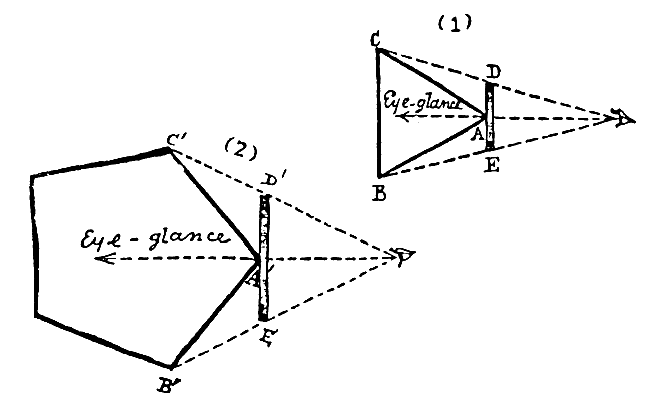
\includegraphics[trim=0mm 0mm 0mm 0mm, width=\linewidth]{fig3}

It will be obvious, to every child in Spaceland who has touched the threshold
of Geometrical Studies, that, if I can bring my eye so that its glance may
bisect an angle (A) of the approaching stranger, my view will lie as it were
evenly between his two sides that are next to me (viz. CA and AB), so that I
shall contemplate the two impartially, and both will appear of the same size.

Now in the case of (1) the Merchant, what shall I see? I shall see a straight
line DAE, in which the middle point (A) will be very bright because it is
nearest to me; but on either side the line will shade away rapidly to dimness,
because the sides AC and AB recede rapidly into the fog and what appear to me
as the Merchant's extremities, viz. D and E, will be very dim indeed.

On the other hand in the case of (2) the Physician, though I shall here also
see a line (D'A'E') with a bright centre (A'), yet it will shade away less
\emph{rapidly into dimness}, because the sides (A'C', A'B') \emph{recede less rapidly into
the fog}: and what appear to me the Physician's extremities, viz. D' and E',
will not be \emph{not so dim} as the extremities of the Merchant.

The Reader will probably understand from these
two instances how --- after a very long training supplemented by constant
experience --- it is possible for the well-educated classes among us to
discriminate with fair accuracy between the middle and lowest orders, by the
sense of sight. If my Spaceland Patrons have grasped this general conception,
so far as to conceive the possibility of it and not to reject my account as
altogether incredible --- I shall have attained all I can reasonably expect.
Were I to attempt further details I should only perplex. Yet for the sake of
the young and inexperienced, who may perchance infer --- from the two simple
instances I have given above, of the manner in which I should recognize my
Father and my Sons --- that Recognition by sight is an easy affair, it may be
needful to point out that in actual life most of the problems of Sight
Recognition are far more subtle and complex.

If for example, when my Father, the Triangle, approaches me, he happens to
present his side to me instead of his angle, then, until I have asked him to
rotate, or until I have edged my eye around him, I am for the moment doubtful
whether he may not be a Straight Line, or, in other words, a Woman. Again,
when I am in the company of one of my two hexagonal Grandsons, contemplating
one of his sides (AB) full front, it will be evident from the accompanying
diagram that I shall see one whole line (AB) in comparative brightness
(shading off hardly at all at the ends) and two smaller lines (CA and BD) dim
throughout and shading away into greater dimness towards the extremities C and
D. 
\begin{center}
    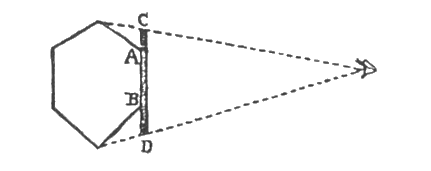
\includegraphics[trim=0mm 0mm 0mm 0mm, scale=0.5]{fig4}
\end{center}


But I must not give way to the temptation of enlarging on these
topics. The meanest mathematician in Spaceland will readily believe me when I
assert that the problems of life, which present themselves to the
well-educated --- when they are themselves in motion, rotating, advancing or
retreating, and at the same time attempting to discriminate by the sense of
sight between a number of Polygons of high rank moving in different
directions, as for example in a ball-room or conversazione --- must be of a
nature to task the angularity of the most intellectual, and amply justify the
rich endowments of the Learned Professors of Geometry, both Static and
Kinetic, in the illustrious University of Wentbridge, where the Science and
Art of Sight Recognition are regularly taught to large classes of the 
\emph{{\'e}lite} of the States.

It is only a few of the scions of our
noblest and wealthiest houses, who are able to give the time and money
necessary for the thorough prosecution of this noble and valuable Art. Even to
me, a Mathematician of no mean standing, and the Grandfather of two most
hopeful and perfectly regular Hexagons, to find myself in the midst of a crowd
of rotating Polygons of the higher classes, is occasionally very perplexing.
And of course to a common Tradesman, or Serf, such a sight is almost as
unintelligible as it would be to you, my Reader, were you suddenly transported
to our country.

In such a crowd you could see on all sides of you nothing but a Line,
apparently straight, but of which the parts would vary irregularly and
perpetually in brightness or dimness. Even if you had completed your third
year in the Pentagonal and Hexagonal classes in the University, and were
perfect in the theory of the subject, you would still find there was need of
many years of experience, before you could move in a fashionable crowd without
jostling against your betters, whom it is against etiquette to ask to ``feel'',
and who, by their superior culture and breeding, know all about your
movements, while you know very little or nothing about theirs. In a word, to
comport oneself with perfect propriety in Polygonal society, one ought to be a
Polygon oneself. Such at least is the painful teaching of my experience.

It is astonishing how much the Art --- or I may almost
call it instinct --- of Sight Recognition is developed by the habitual practice
of it and by the avoidance of the custom of ``Feeling''. Just as, with you, the
deaf and dumb, if once allowed to gesticulate and to use the hand-alphabet,
will never acquire the more difficult but far more valuable art of lip-speech
and lip-reading, so it is with us as regards ``Seeing'' and ``Feeling''. None who
in early life resort to ``Feeling'' will ever learn ``Seeing'' in perfection.

For this reason, among our Higher Classes, ``Feeling'' is discouraged or
absolutely forbidden. From the cradle their children, instead of going to the
Public Elementary schools (where the art of Feeling is taught,) are sent to
higher Seminaries of an exclusive character; and at our illustrious
University, to ``feel'' is regarded as a most serious fault, involving
Rustication for the first offence, and Expulsion for the second.

But among the lower classes the art of Sight Recognition is regarded as an
unattainable luxury. A common Tradesman cannot afford to let his son spend a
third of his life in abstract studies. The children of the poor are therefore
allowed to ``feel'' from their earliest years, and they gain thereby a precocity
and an early vivacity which contrast at first most favourably with the inert,
undeveloped, and listless behaviour of the half-instructed youths of the
Polygonal class; but when the latter have at last completed their University
course, and are prepared to put their theory into practice, the change that
comes over them may almost be described as a new birth, and in every art,
science, and social pursuit they rapidly overtake and distance their
Triangular competitors.

Only a few of the Polygonal Class fail to pass the Final Test or Leaving
Examination at the University. The condition of the unsuccessful minority is
truly pitiable.  Rejected from the higher class, they are also despised by the
lower. They have neither the matured and systematically trained powers of the
Polygonal Bachelors and Masters of Arts, nor yet the native precocity and
mercurial versatility of the youthful Tradesman. The professions, the public
services, are closed against them, and though in most States they are not
actually debarred from marriage, yet they have the greatest difficulty in
forming suitable alliances, as experience shews that the offspring of such
unfortunate and ill-endowed parents is generally itself unfortunate, if not
positively Irregular.

It is from these specimens of the refuse of our Nobility that the great
Tumults and Seditions of past ages have generally derived their leaders; and
so great is the mischief thence arising that an increasing minority of our
more progressive Statesmen are of opinion that true mercy would dictate their
entire suppression, by enacting that all who fail to pass the Final
Examination of the University should be either imprisoned for life, or
extinguished by a painless death.

But I find myself digressing into the subject of Irregularities, a matter of
such vital interest that it demands a separate section.


\chapter{Concerning Irregular Figures}


Throughout the previous pages I have been assuming --- what perhaps should have
been laid down at the beginning as a distinct and fundamental proposition ---
that every human being in Flatland is a Regular Figure, that is to say of
regular construction. By this I mean that a Woman must not only be a line, but
a straight line; that an Artisan or Soldier must have two of his sides equal;
that Tradesmen must have three sides equal; Lawyers (of which class I am a
humble member), four sides equal, and, generally, that in every Polygon, all
the sides must be equal.

The sizes of the sides would of course depend upon the age of the individual.
A Female at birth would be about an inch long, while a tall adult Woman might
extend to a foot. As to the Males of every class, it may be roughly said that
the length of an adult's size, when added together, is two feet or a little
more. But the size of our sides is not under consideration. I am speaking of
the \emph{equality} of sides, and it does not need much reflection to see that the
whole of the social life in Flatland rests upon the fundamental fact that
Nature wills all Figures to have their sides equal.

If our sides were unequal our angles might be unequal. Instead of its being
sufficient to feel, or estimate by sight, a single angle in order to determine
the form of an individual, it would be necessary to ascertain each angle by
the experiment of Feeling. But life would be too short for such a tedious
groping. The whole science and art of Sight Recognition would at once perish;
Feeling, so far as it is an art, would not long survive; intercourse would
become perilous or impossible; there would be an end to all confidence, all
forethought; no one would be safe in making the most simple social
arrangements; in a word, civilization might relapse into barbarism.

Am I going too fast to carry my Readers with me to these obvious conclusions?
Surely a moment's reflection, and a single instance from common life, must
convince every one that our social system is based upon Regularity, or
Equality of Angles. You meet, for example, two or three Tradesmen in the
street, whom your recognize at once to be Tradesman by a glance at their
angles and rapidly bedimmed sides, and you ask them to step into your house to
lunch. This you do at present with perfect confidence, because everyone knows
to an inch or two the area occupied by an adult Triangle: but imagine that
your Tradesman drags behind his regular and respectable vertex, a
parallelogram of twelve or thirteen inches in diagonal: --- what are you to do
with such a monster sticking fast in your house door?

But I am insulting the intelligence of my Readers by accumulating details
which must be patent to everyone who enjoys the advantages of a Residence in
Spaceland. Obviously the measurements of a single angle would no longer be
sufficient under such portentous circumstances; one's whole life would be
taken up in feeling or surveying the perimeter of one's acquaintances. Already
the difficulties of avoiding a collision in a crowd are enough to tax the
sagacity of even a well-educated Square; but if no one could calculate the
Regularity of a single figure in the company, all would be chaos and
confusion, and the slightest panic would cause serious injuries, or --- if there
happened to be any Women or Soldiers present --- perhaps considerable loss of
life.

Expediency therefore concurs with Nature in stamping the seal of its approval
upon Regularity of conformation: nor has the Law been backward in seconding
their efforts. ``Irregularity of Figure'' means with us the same as, or more
than, a combination of moral obliquity and criminality with you, and is
treated accordingly. There are not wanting, it is true, some promulgators of
paradoxes who maintain that there is no necessary connection between
geometrical and moral Irregularity. ``The Irregular,'' they say, ``is from his
birth scouted by his own parents, derided by his brothers and sisters,
neglected by the domestics, scorned and suspected by society, and excluded
from all posts of responsibility, trust, and useful activity. His every
movement is jealously watched by the police till he comes of age and presents
himself for inspection; then he is either destroyed, if he is found to exceed
the fixed margin of deviation, at an uninteresting occupation for a miserable
stipend; obliged to live and board at the office, and to take even his
vacation under close supervision; what wonder that human nature, even in the
best and purest, is embittered and perverted by such surroundings!''

All this very plausible reasoning does not convince me, as it has not
convinced the wisest of our Statesmen, that our ancestors erred in laying it
down as an axiom of policy that the toleration of Irregularity is incompatible
with the safety of the State. Doubtless, the life of an Irregular is hard; but
the interests of the Greater Number require that it shall be hard. If a man
with a triangular front and a polygonal back were allowed to exist and to
propagate a still more Irregular posterity, what would become of the arts of
life? Are the houses and doors and churches in Flatland to be altered in order
to accommodate such monsters? Are our ticket-collectors to be required to
measure every man's perimeter before they allow him to enter a theatre, or to
take his place in a lecture room? Is an Irregular to be exempted from the
militia? And if not, how is he to be prevented from carrying desolation into
the ranks of his comrades? Again, what irresistible temptations to fraudulent
impostures must needs beset such a creature! How easy for him to enter a shop
with his polygonal front foremost, and to order goods to any extent from a
confiding tradesman! Let the advocates of a falsely called Philanthropy plead
as they may for the abrogation of the Irregular Penal Laws, I for my part have
never known an Irregular who was not also what Nature evidently intended him
to be --- a hypocrite, a misanthropist, and, up to the limits of his power, a
perpetrator of all manner of mischief.

Not that I should be disposed to recommend (at present) the extreme measures
adopted by some States, where an infant whose angle deviates by half a degree
from the correct angularity is summarily destroyed at birth.  Some of our
highest and ablest men, men of real genius, have during their earliest days
laboured under deviations as great as, or even greater than forty-five
minutes: and the loss of their precious lives would have been an irreparable
injury to the State. The art of healing also has achieved some of its most
glorious triumphs in the compressions, extensions, trepannings, colligations,
and other surgical or di{\ae}tetic operations by which Irregularity has been
partly or wholly cured. Advocating therefore a \emph{Via Media}, I would lay down no
fixed or absolute line of demarcation; but at the period when the frame is
just beginning to set, and when the Medical Board has reported that recovery
is improbably, I would suggest that the Irregular offspring be painlessly and
mercifully consumed.


\chapter{Of the Ancient Practice of Painting}


If my Readers have followed me with any attention up to this point, they will
not be surprised to hear that life is somewhat dull in Flatland. I do not, of
course, mean that there are not battles, conspiracies, tumults, factions, and
all those other phenomena which are supposed to make History interesting; nor
would I deny that the strange mixture of the problems of life and the problems
of Mathematics, continually inducing conjecture and giving an opportunity of
immediate verification, imparts to our existence a zest which you in Spaceland
can hardly comprehend. I speak now from the aesthetic and artistic point of
view when I say that life with us is dull; aesthetically and artistically,
very dull indeed.

How can it be otherwise, when all one's prospect, all one's landscapes,
historical pieces, portraits, flowers, still life, are nothing but a single
line, with no varieties except degrees of brightness and obscurity?

It was not always thus. Colour, if Tradition speaks the truth, once for the
space of half a dozen centuries or more, threw a transient splendour over the
lives of our ancestors in the remotest ages. Some private individual --- a
Pentagon whose name is variously reported --- having casually discovered the
constituents of the simpler colours and a rudimentary method of painting, is
said to have begun by decorating first his house, then his slaves, then his
Father, his Sons, and Grandsons, lastly himself. The convenience as well as
the beauty of the results commended themselves to all. Wherever Chromatistes,
--- for by that name the most trustworthy authorities concur in calling him, ---
turned his variegated frame, there he at once excited attention, and attracted
respect. No one now needed to ``feel'' him; no one mistook his front for his
back; all his movements were readily ascertained by his neighbours without the
slightest strain on their powers of calculation; no one jostled him, or failed
to make way for him; his voice was saved the labour of that exhausting
utterance by which we colourless Squares and Pentagons are often forced to
proclaim our individuality when we move amid a crowd of ignorant Isosceles.

The fashion spread like wildfire. Before a week was over, every Square and
Triangle in the district had copied the example of Chromatistes, and only a
few of the more conservative Pentagons still held out. A month or two found
even the Dodecagons infected with the innovation. A year had not elapsed
before the habit had spread to all but the very highest of the Nobility.
Needless to say, the custom soon made its way from the district of
Chromatistes to surrounding regions; and within two generations no one in all
Flatland was colourless except the Women and the Priests.

Here Nature herself appeared to erect a barrier, and to plead against
extending the innovations to these two classes. Many-sidedness was almost
essential as a pretext for the Innovators. ``Distinction of sides is intended
by Nature to imply distinction of colours'' --- such was the sophism which in
those days flew from mouth to mouth, converting whole towns at a time to a new
culture. But manifestly to our Priests and Women this adage did not apply. The
latter had only one side, and therefore --- plurally and pedantically speaking ---
\emph{no sides}. The former --- if at least they would assert their claim to be readily
and truly Circles, and not mere high-class Polygons, with an infinitely large
number of infinitesimally small sides --- were in the habit of boasting (what
Women confessed and deplored) that they also had no sides, being blessed with
a perimeter of only one line, or, in other words, a Circumference. Hence it
came to pass that these two Classes could see no force in the so-called axiom
about ``Distinction of Sides implying Distinction of Colour;'' and when all
others had succumbed to the fascinations of corporal decoration, the Priests
and the Women alone still remained pure from the pollution of paint.

Immoral, licentious, anarchical, unscientific --- call them by what names you
will --- yet, from an aesthetic point of view, those ancient days of the Colour
Revolt were the glorious childhood of Art in Flatland --- a childhood, alas,
that never ripened into manhood, nor even reached the blossom of youth. To
live then in itself a delight, because living implied seeing. Even at a small
party, the company was a pleasure to behold; the richly varied hues of the
assembly in a church or theatre are said to have more than once proved too
distracting from our greatest teachers and actors; but most ravishing of all
is said to have been the unspeakable magnificence of a military review.

The sight of a line of battle of twenty thousand
Isosceles suddenly facing about, and exchanging the sombre black of their
bases for the orange of the two sides including their acute angle; the militia
of the Equilateral Triangles tricoloured in red, white, and blue; the mauve,
ultra-marine, gamboge, and burnt umber of the Square artillerymen rapidly
rotating near their vermillion guns; the dashing and flashing of the
five-coloured and six-coloured Pentagons and Hexagons careering across the
field in their offices of surgeons, geometricians and aides-de-camp --- all
these may well have been sufficient to render credible the famous story how an
illustrious Circle, overcome by the artistic beauty of the forces under his
command, threw aside his marshal's baton and his royal crown, exclaiming that
he henceforth exchanged them for the artist's pencil. How great and glorious
the sensuous development of these days must have been is in part indicated by
the very language and vocabulary of the period. The commonest utterances of
the commonest citizens in the time of the Colour Revolt seem to have been
suffused with a richer tinge of word or thought; and to that era we are even
now indebted for our finest poetry and for whatever rhythm still remains in
the more scientific utterance of those modern days.


\chapter{Of the Universal Colour Bill}


But meanwhile the intellectual Arts were fast decaying.
The Art of Sight Recognition, being no longer needed, was no longer practised;
and the studies of Geometry, Statics, Kinetics, and other kindred subjects,
came soon to be considered superfluous, and fell into disrespect and neglect
even at our University. The inferior Art of Feeling speedily experienced the
same fate at our Elementary Schools. Then the Isosceles classes, asserting
that the Specimens were no longer used nor needed, and refusing to pay the
customary tribute from the Criminal classes to the service of Education, waxed
daily more numerous and more insolent on the strength of their immunity from
the old burden which had formerly exercised the twofold wholesome effect of at
once taming their brutal nature and thinning their excessive numbers.

Year by year the Soldiers and Artisans began more vehemently to assert --- and
with increasing truth --- that there was no great difference between them and
the very highest class of Polygons, now that they were raised to an equality
with the latter, and enabled to grapple with all the difficulties and solve
all the problems of life, whether Statical or Kinetical, by the simple process
of Colour Recognition. Not content with the natural neglect into which Sight
Recognition was falling, they began boldly to demand the legal prohibition of
all ``monopolizing and aristocratic Arts'' and the consequent abolition of all
endowments for the studies of Sight Recognition, Mathematics, and Feeling.
Soon, they began to insist that inasmuch as Colour, which was a second Nature,
had destroyed the need of aristocratic distinctions, the Law should follow in
the same path, and that henceforth all individuals and all classes should be
recognized as absolutely equal and entitled to equal rights.

Finding the higher Orders wavering and undecided, the leaders of the
Revolution advanced still further in their requirements, and at last demanded
that all classes alike, the Priests and the Women not excepted, should do
homage to Colour by submitting to be painted. When it was objected that
Priests and Women had no sides, they retorted that Nature and Expediency
concurred in dictating that the front half of every human being (that is to
say, the half containing his eye and mouth) should be distinguishable from his
hinder half. They therefore brought before a general and extraordinary
Assembly of all the States of Flatland a Bill proposing that in every Woman
the half containing the eye and mouth should be coloured red, and the other
half green. The Priests were to be painted in the same way, red being applied
to that semicircle in which the eye and mouth formed the middle point; while
the other or hinder semicircle was to be coloured green.

There was no little cunning in this proposal, which indeed emanated not from
any Isosceles --- for no being so degraded would have angularity enough to
appreciate, much less to devise, such a model of state-craft --- but from an
Irregular Circle who, instead of being destroyed in his childhood, was
reserved by a foolish indulgence to bring desolation on his country and
destruction on myriads of followers.

On the one hand the proposition was calculated to bring the Women in all
classes over to the side of the Chromatic Innovation. For by assigning to the
Women the same two colours as were assigned to the Priests, the Revolutionists
thereby ensured that, in certain positions, every Woman would appear as a
Priest, and be treated with corresponding respect and deference --- a prospect
that could not fail to attract the Female Sex in a mass.

But by some of my Readers the possibility of the identical appearance of
Priests and Women, under a new Legislation, may not be recognized; if so, a
word or two will make it obvious.

Imagine a woman duly decorated, according to the new Code; with the front half
(i.e., the half containing the eye and mouth) red, and with the hinder half
green. Look at her from one side. Obviously you will see a straight line, \emph{half
red}, \emph{half green}. 
\begin{center}
    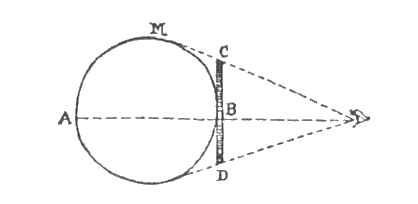
\includegraphics[trim=0mm 0mm 0mm 0mm, scale=0.5]{fig5}
\end{center}

Now imagine a Priest, whose mouth is at M, and whose front semicircle (AMB) is
consequently coloured red, while his hinder semicircle is green; so that the
diameter AB divides the green from the red. If you contemplate the Great Man
so as to have your eye in the same straight line as his dividing diameter
(AB), what you will see will be a straight line (CBD), of which \emph{one half} (CB)
\emph{will be red}, \emph{and the other} (BD) \emph{green}. The whole line (CD) will be rather
shorter perhaps than that of a full-sized Woman, and will shade off more
rapidly towards its extremities; but the identity of the colours would give
you an immediate impression of identity in Class, making you neglectful of
other details. Bear in mind the decay of Sight Recognition which threatened
society at the time of the Colour revolt; add too the certainty that Woman
would speedily learn to shade off their extremities so as to imitate the
Circles; it must then be surely obvious to you, my dear Reader, that the
Colour Bill placed us under a great danger of confounding a Priest with a
young Woman.

How attractive this prospect must have been to the Frail Sex may readily be
imagined. They anticipated with delight the confusion that would ensue. At
home they might hear political and ecclesiastical secrets intended not for
them but for their husbands and brothers, and might even issue some commands
in the name of a priestly Circle; out of doors the striking combination of red
and green without addition of any other colours, would be sure to lead the
common people into endless mistakes, and the Woman would gain whatever the
Circles lost, in the deference of the passers by. As for the scandal that
would befall the Circular Class if the frivolous and unseemly conduct of the
Women were imputed to them, and as to the consequent subversion of the
Constitution, the Female Sex could not be expected to give a thought to these
considerations. Even in the households of the Circles, the Women were all in
favour of the Universal Colour Bill.

The second object aimed at by the Bill was the gradual demoralization of the
Circles themselves. In the general intellectual decay they still preserved
their pristine clearness and strength of understanding. From their earliest
childhood, familiarized in their Circular households with the total absence of
Colour, the Nobles alone preserved the Sacred Art of Sight Recognition, with
all the advantages that result from that admirable training of the intellect.
Hence, up to the date of the introduction of the Universal Colour Bill, the
Circles had not only held their own, but even increased their lead of the
other classes by abstinence from the popular fashion.

Now therefore the artful Irregular whom I described above as the real author
of this diabolical Bill, determined at one blow to lower the status of the
Hierarchy by forcing them to submit to the pollution of Colour, and at the
same time to destroy their domestic opportunities of training in the Art of
Sight Recognition, so as to enfeeble their intellects by depriving them of
their pure and colourless homes. Once subjected to the chromatic taint, every
parental and every childish Circle would demoralize each other. Only in
discerning between the Father and the Mother would the Circular infant find
problems for the exercise of his understanding --- problems too often likely to
be corrupted by maternal impostures with the result of shaking the child's
faith in all logical conclusions. Thus by degrees the intellectual lustre of
the Priestly Order would wane, and the road would then lie open for a total
destruction of all Aristocratic Legislature and for the subversion of our
Privileged Classes.


\chapter{Of the Suppression of the Chromatic Sedition}
The agitation for the Universal Colour Bill continued for three years; and up
to the last moment of that period it seemed as though Anarchy were destined to
triumph.

A whole army of Polygons, who turned out to fight as private soldiers, was
utterly annihilated by a superior force of Isosceles Triangles --- the Squares
and Pentagons meanwhile remaining neutral. Worse than all, some of the ablest
Circles fell a prey to conjugal fury. Infuriated by political animosity, the
wives in many a noble household wearied their lords with prayers to give up
their opposition to the Colour Bill; and some, finding their entreaties
fruitless, fell on and slaughtered their innocent children and husband,
perishing themselves in the act of carnage. It is recorded that during that
triennial agitation no less than twenty-three Circles perished in domestic
discord.

Great indeed was the peril. It seemed as though the Priests had no choice
between submission and extermination; when suddenly the course of events was
completely changed by one of those picturesque incidents which Statesmen ought
never to neglect, often to anticipate, and sometimes perhaps to originate,
because of the absurdly disproportionate power with which they appeal to the
sympathies of the populace.

It happened that an Isosceles of a low type, with a brain little if at all
above four degrees --- accidentally dabbling in the colours of some Tradesman
whose shop he had plundered --- painted himself, or caused himself to be painted
(for the story varies) with the twelve colours of a Dodecagon. Going into the
Market Place he accosted in a feigned voice a maiden, the orphan daughter of a
noble Polygon, whose affection in former days he had sought in vain; and by a
series of deceptions --- aided, on the one side, by a string of lucky accidents
too long to relate, and, on the other, by an almost inconceivable fatuity and
neglect of ordinary precautions on the part of the relations of the bride --- he
succeeded in consummating the marriage. The unhappy girl committed suicide on
discovering the fraud to which she had been subjected.

When the news of this catastrophe spread from State to State the minds of the
Women were violently agitated. Sympathy with the miserable victim and
anticipations of similar deceptions for themselves, their sisters, and their
daughters, made them now regard the Colour Bill in an entirely new aspect. Not
a few openly avowed themselves converted to antagonism; the rest needed only a
slight stimulus to make a similar avowal. Seizing this favourable opportunity,
the Circles hastily convened an extraordinary Assembly of the States; and
besides the usual guard of Convicts, they secured the attendance of a large
number of reactionary Women.

Amidst an unprecedented concourse, the Chief Circle of those days --- by name
Pantocyclus --- arose to find himself hissed and hooted by a hundred and twenty
thousand Isosceles. But he secured silence by declaring that henceforth the
Circles would enter on a policy of Concession; yielding to the wishes of the
majority, they would accept the Colour Bill. The uproar being at once
converted to applause, he invited Chromatistes, the leader of the Sedition,
into the centre of the hall, to receive in the name of his followers the
submission of the Hierarchy. Then followed a speech, a masterpiece of
rhetoric, which occupied nearly a day in the delivery, and to which no summary
can do justice.

With a grave appearance of impartiality he declared that as they were now
finally committing themselves to Reform or Innovation, it was desirable that
they should take one last view of the perimeter of the whole subject, its
defects as well as its advantages. Gradually introduction the mention of the
dangers to the Tradesmen, the Professional Classes and the Gentlemen, he
silenced the rising murmurs of the Isosceles by reminding them that, in spite
of all these defects, he was willing to accept the Bill if it was approved by
the majority. But it was manifest that all, except the Isosceles, were moved
by his words and were either neutral or averse to the Bill.

Turning now to the Workmen he asserted that their interests must not be
neglected, and that, if they intended to accept the Colour Bill, they ought at
least to do so with full view of the consequences. Many of them, he said, were
on the point of being admitted to the class of the Regular Triangles; others
anticipated for their children a distinction they could not hope for
themselves. That honourable ambition would now have to be sacrificed. With the
universal adoption of Colour, all distinctions would cease; Regularity would
be confused with Irregularity; development would give place to retrogression;
the Workman would in a few generations be degraded to the level of the
Military, or even the Convict Class; political power would be in the hands of
the greatest number, that is to say the Criminal Classes, who were already
more numerous than the Workmen, and would soon out-number all the other
Classes put together when the usual Compensative Laws of Nature were violated.

A subdued murmur of assent ran through the ranks of the Artisans, and
Chromatistes, in alarm, attempted to step forward and address them. But he
found himself encompassed with guards and forced to remain silent while the
Chief Circle in a few impassioned words made a final appeal to the Women,
exclaiming that, if the Colour Bill passed, no marriage would henceforth be
safe, no woman's honour secure; fraud, deception, hypocrisy would pervade
every household; domestic bliss would share the fate of the Constitution and
pass to speedy perdition. ``Sooner than this'', he cried, ``Come death''.

At these words, which were the preconcerted signal for action, the Isosceles
Convicts fell on and transfixed the wretched Chromatistes; the Regular
Classes, opening their ranks, made way for a band of Women who, under
direction of the Circles, moved back foremost, invisibly and unerringly upon
the unconscious soldiers; the Artisans, imitating the example of their
betters, also opened their ranks. Meantime bands of Convicts occupied every
entrance with an impenetrable phalanx.

The battle, or rather carnage, was of short duration. Under the skillful
generalship of the Circles almost every Woman's charge was fatal and very many
extracted their sting uninjured, ready for a second slaughter. But no second
blow was needed; the rabble of the Isosceles did the rest of the business for
themselves. Surprised, leader-less, attacked in front by invisible foes, and
finding egress cut off by the Convicts behind them, they at once --- after their
manner --- lost all presence of mind, and raised the cry of ``treachery''. This
sealed their fate. Every Isosceles now saw and felt a foe in every other. In
half an hour not one of that vast multitude was living; and the fragments of
seven score thousand of the Criminal Class slain by one another's angles
attested the triumph of Order.

The Circles delayed not to push their victory to the uttermost. The Working
Men they spared but decimated. The Militia of the Equilaterals was at once
called out, and every Triangle suspected of Irregularity on reasonable
grounds, was destroyed by Court Martial, without the formality of exact
measurement by the Social Board. The homes of the Military and Artisan classes
were inspected in a course of visitation extending through upwards of a year;
and during that period every town, village, and hamlet was systematically
purged of that excess of the lower orders which had been brought about by the
neglect to pay the tribute of Criminals to the Schools and University, and by
the violation of other natural Laws of the Constitution of Flatland. Thus the
balance of classes was again restored.

Needless to say that henceforth the use of Colour was abolished, and its
possession prohibited. Even the utterance of any word denoting Colour, except
by the Circles or by qualified scientific teachers, was punished by a severe
penalty. Only at our University in some of the very highest and most esoteric
classes --- which I myself have never been privileged to attend --- it is
understood that the sparing use of Colour is still sanctioned for the purpose
of illustrating some of the deeper problems of mathematics. But of this I can
only speak from hearsay.

Elsewhere in Flatland, Colour is now non-existent. The art of making it is
known to only one living person, the Chief Circle for the time being; and by
him it is handed down on his death-bed to none but his Successor. One
manufactory alone produces it; and, lest the secret should be betrayed, the
Workmen are annually consumed, and fresh ones introduced. So great is the
terror with which even now our Aristocracy looks back to the far-distant days
of the agitation for the Universal Colour Bill.


\chapter{Concerning our Priests}


It is high time that I should pass from these brief and discursive notes about
things in Flatland to the central event of this book, my initiation into the
mysteries of Space. That is my subject; all that has gone before is merely
preface.

For this reason I must omit many matters of which the explanation would not, I
flatter myself, be without interest for my Readers: as for example, our method
of propelling and stopping ourselves, although destitute of feet; the means by
which we give fixity to structures of wood, stone, or brick, although of
course we have no hands, nor can we lay foundations as you can, nor avail
ourselves of the lateral pressure of the earth; the manner in which the rain
originates in the intervals between our various zones, so that the northern
regions do not intercept the moisture falling on the southern; the nature of
our hills and mines, our trees and vegetables, our seasons and harvests; our
Alphabet and method of writing, adapted to our linear tablets; these and a
hundred other details of our physical existence I must pass over, nor do I
mention them now except to indicate to my readers that their omission proceeds
not from forgetfulness on the part of the author, but from his regard for the
time of the Reader.

Yet before I proceed to my legitimate subject some few final remarks will no
doubt be expected by my Readers upon these pillars and mainstays of the
Constitution of Flatland, the controllers of our conduct and shapers of our
destiny, the objects of universal homage and almost of adoration: need I say
that I mean our Circles or Priests?

When I call them Priests, let me not be understood as meaning no more than the
term denotes with you. With us, our Priests are Administrators of all
Business, Art, and Science; Directors of Trade, Commerce, Generalship,
Architecture, Engineering, Education, Statesmanship, Legislature, Morality,
Theology; doing nothing themselves, they are the Causes of everything worth
doing, that is done by others.

Although popularly everyone called a Circle is deemed a Circle, yet among the
better educated Classes it is known that no Circle is really a Circle, but
only a Polygon with a very large number of very small sides. As the number of
the sides increases, a Polygon approximates to a Circle; and, when the number
is very great indeed, say for example three or four hundred, it is extremely
difficult for the most delicate touch to feel any polygonal angles. Let me say
rather it \emph{would} be difficult: for, as I have shown above, Recognition by
Feeling is unknown among the highest society, and to \emph{feel} a Circle would be
considered a most audacious insult. This habit of abstention from Feeling in
the best society enables a Circle the more easily to sustain the veil of
mystery in which, from his earliest years, he is wont to enwrap the exact
nature of his Perimeter or Circumference. Three feet being the average
Perimeter it follows that, in a Polygon of three hundred sides each side will
be no more than the hundredth part of a foot in length, or little more than
the tenth part of an inch; and in a Polygon of six or seven hundred sides the
sides are little larger than the diameter of a Spaceland pin-head. It is
always assumed, by courtesy, that the Chief Circle for the time being has ten
thousand sides.

The ascent of the posterity of the Circles in the social scale is not
restricted, as it is among the lower Regular classes, by the Law of Nature
which limits the increase of sides to one in each generation. If it were so,
the number of sides in the Circle would be a mere question of pedigree and
arithmetic, and the four hundred and ninety-seventh descendant of an
Equilateral Triangle would necessarily be a polygon With five hundred sides.
But this is not the case. Nature's Law prescribes two antagonistic decrees
affecting Circular propagation; first, that as the race climbs higher in the
scale of development, so development shall proceed at an accelerated pace;
second, that in the same proportion, the race shall become less fertile.
Consequently in the home of a Polygon of four or five hundred sides it is rare
to find a son; more than one is never seen. On the other hand the son of a
five-hundred-sided Polygon has been known to possess five hundred and fifty,
or even six hundred sides.

Art also steps in to help the process of higher Evolution. Our physicians have
discovered that the small and tender sides of an infant Polygon of the higher
class can be fractured, and his whole frame re-set, with such exactness that a
Polygon of two or three hundred sides sometimes --- by no means always, for the
process is attended with serious risk --- but sometimes overleaps two or three
hundred generations, and as it were double at a stroke, the number of his
progenitors and the nobility of his descent.

Many a promising child is sacrificed in this way. Scarcely one out of ten
survives. Yet so strong is the parental ambition among those Polygons who are,
as it were, on the fringe of the Circular class, that it is very rare to find
the Nobleman of that position in society, who has neglected to place his
first-born in the Circular Neo-Therapeutic Gymnasium before he has attained
the age of a month.

One year determines success or failure. At the end of that time the child has,
in all probability, added one more to the tombstones that crowd the
Neo-Therapeutic Cemetery; but on rare occasional a glad procession bares back
the little one to his exultant parents, no longer a Polygon, but a Circle, at
least by courtesy: and a single instance of so blessed a result induces
multitudes of Polygonal parents to submit to similar domestic sacrifice, which
have a dissimilar issue.


\chapter{Of the Doctrine of our Priests}


As to the doctrine of the Circles it may briefly be summed up in a single
maxim, ``Attend to your Configuration''. Whether political, ecclesiastical, or
moral, all their teaching has for its object the improvement of individual and
collective Configuration --- with special reference of course to the
Configuration of the Circles, to which all other objects are subordinated.

It is the merit of the Circles that they have effectually suppressed those
ancient heresies which led men to waste energy and sympathy in the vain belief
that conduct depends upon will, effort, training, encouragement, praise, or
anything else but Configuration. It was Pantocyclus --- the illustrious Circle
mentioned above, as the queller of the Colour Revolt --- who first convinced
mankind that Configuration makes the man; that if, for example, you are born
an Isosceles with two uneven sides, you will assuredly go wrong unless you
have them made even --- for which purpose you must go to the Isosceles Hospital;
similarly, if you are a Triangle, or Square, or even a Polygon, born with any
Irregularity, you must be taken to one of the Regular Hospitals to have your
disease cured; otherwise you will end your days in the State Prison or by the
angle of the State Executioner.

All faults or defects, from the slightest misconduct to the most flagitious
crime, Pantocyclus attributed to some deviation from perfect Regularity in the
bodily figure, caused perhaps (if not congenital by some collision in a crowd;
by neglect to take exercise, or by taking too much of it; or even by a sudden
change of temperature, resulting in a shrinkage or expansion in some too
susceptible part of the frame. Therefore, concluded that illustrious
Philosopher, neither good conduct nor bad conduct is a fit subject, in any
sober estimation, for either praise or blame. For why should you praise, for
example, the integrity of a Square who faithfully defends the interests of his
client, when you ought in reality rather to admire the exact precision of his
right angles? Or again, why blame a lying, thievish Isosceles, when you ought
rather to deplore the incurable inequality of his sides?

Theoretically, this doctrine is unquestionable; but it has practical
drawbacks. In dealing with an Isosceles, if a rascal pleads that he cannot
help stealing because of his unevenness, you reply that for that very reason,
because he cannot help being a nuisance to his neighbours, you, the
Magistrate, cannot help sentencing him to be consumed --- and there's an end of
the matter. But in little domestic difficulties, when the penalty of
consumption, or death, is out of the question, this theory of Configuration
sometimes comes in awkwardly; and I must confess that occasionally when one of
my own Hexagonal Grandsons pleads as an excuse for his disobedience that a
sudden change of temperature has been too much for his Perimeter, and that I
ought to lay the blame not on him but on his Configuration, which can only be
strengthened by abundance of the choicest sweetmeats, I neither see my way
logically to reject, nor practically to accept, his conclusions.

For my own part, I find it best to assume that a good sound scolding or
castigation has some latent and strengthening influence on my Grandson's
Configuration; though I own that I have no grounds for thinking so. At all
events I am not alone in my way of extricating myself from this dilemma; for I
find that many of the highest Circles, sitting as Judges in law courts, use
praise and blame towards Regular and Irregular Figures; and in their homes I
know by experience that, when scolding their children, they speak about
``right'' and ``wrong'' as vehemently and passionately as if they believe that
these names represented real existence, and that a human Figure is really
capable of choosing between them.

Constantly carrying out their policy of making Configuration the leading idea
in every mind, the Circles reverse the nature of that Commandment which in
Spaceland regulates the relations between parents and children. With you,
children are taught to honour their parents; with us --- next to the Circles,
who are the chief object of universal homage --- a man is taught to honour his
Grandson, if he has one; or, if not, his Son. By ``honour'', however, is by no
means mean ``indulgence'', but a reverent regard for their highest interests:
and the Circles teach that the duty of fathers is to subordinate their own
interests to those of posterity, thereby advancing the welfare of the whole
State as well as that of their own immediate descendants.

The weak point in the system of the Circles --- if a humble Square may venture
to speak of anything Circular as containing any element of weakness --- appears
to me to be found in their relations with Women.

As it is of the utmost importance for Society that Irregular births should be
discouraged, it follows that no Woman who has any Irregularities in her
ancestry is a fit partner for one who desires that his posterity should rise
by regular degrees in the social scale.

Now the Irregularity of a Male is a matter of measurement; but as all Women
are straight, and therefore visibly Regular so to speak, one has to device
some other means of ascertaining what I may call their invisible Irregularity,
that is to say their potential Irregularities as regards possible offspring.
This is effected by carefully-kept pedigrees, which are preserved and
supervised by the State; and without a certified pedigree no Woman is allowed
to marry.

Now it might have been supposed that a Circle --- proud of his ancestry and
regardful for a posterity which might possibly issue hereafter in a Chief
Circle --- would be more careful than any other to choose a wife who had no blot
on her escutcheon. But it is not so. The care in choosing a Regular wife
appears to diminish as one rises in the social scale. Nothing would induce an
aspiring Isosceles, who has hopes of generating an Equilateral Son, to take a
wife who reckoned a single Irregularity among her Ancestors; a Square or
Pentagon, who is confident that his family is steadily on the rise, does not
inquire above the five-hundredth generation; a Hexagon or Dodecagon is even
more careless of the wife's pedigree; but a Circle has been known deliberately
to take a wife who has had an Irregular Great-Grandfather, and all because of
some slight superiority of lustre, or because of the charms of a low voice ---
which, with us, even more than with you, is thought ``an excellent thing in a
Woman''.

Such ill-judged marriages are, as might be expected, barren, if they do not
result in positive Irregularity or in diminution of sides; but none of these
evils have hitherto provided sufficiently deterrent. The loss of a few sides
in a highly-developed Polygon is not easily noticed, and is sometimes
compensated by a successful operation in the Neo-Therapeutic Gymnasium, as I
have described above; and the Circles are too much disposed to acquiesce in
infecundity as a law of the superior development. Yet, if this evil be not
arrested, the gradual diminution of the Circular class may soon become more
rapid, and the time may not be far distant when, the race being no longer able
to produce a Chief Circle, the Constitution of Flatland must fall.

One other word of warning suggest itself to me, though I cannot so easily
mention a remedy; and this also refers to our relations with Women. About
three hundred years ago, it was decreed by the Chief Circle that, since women
are deficient in Reason but abundant in Emotion, they ought no longer to be
treated as rational, nor receive any mental education. The consequence was
that they were no longer taught to read, nor even to master Arithmetic enough
to enable them to count the angles of their husband or children; and hence
they sensibly declined during each generation in intellectual power. And this
system of female non-education or quietism still prevails.

My fear is that, with the best intentions, this policy has been carried so far
as to react injuriously on the Male Sex.

For the consequence is that, as things now are, we Males have to lead a kind
of bi-lingual, and I may almost say bi-mental, existence. With Women, we speak
of ``love'', ``duty'', ``right'', ``wrong'', ``pity'', ``hope'', and other irrational and
emotional conceptions, which have no existence, and the fiction of which has
no object except to control feminine exuberances; but among ourselves, and in
our books, we have an entirely different vocabulary and I may also say, idiom.
``Love'' them becomes ``the anticipation of benefits''; ``duty'' becomes ``necessity''
or ``fitness''; and other words are correspondingly transmuted. Moreover, among
Women, we use language implying the utmost deference for their Sex; and they
fully believe that the Chief Circle Himself is not more devoutly adored by us
than they are: but behind their backs they are both regarded and spoken of ---
by all but the very young --- as being little better than ``mindless organisms''.

Our Theology also in the Women's chambers is entirely different from our
Theology elsewhere.

Now my humble fear is that this double training, in language as well as in
thought, imposes somewhat too heavy a burden upon the young, especially when,
at the age of three years old, they are taken from the maternal care and
taught to unlearn the old language --- except for the purpose of repeating it in
the presence of the Mothers and Nurses --- and to learn the vocabulary and idiom
of science. Already methinks I discern a weakness in the grasp of mathematical
truth at the present time as compared with the more robust intellect of our
ancestors three hundred years ago. I say nothing of the possible danger if a
Woman should ever surreptitiously learn to read and convey to her Sex the
result of her perusal of a single popular volume; nor of the possibility that
the indiscretion or disobedience of some infant Male might reveal to a Mother
the secrets of the logical dialect. On the simple ground of the enfeebling of
the male intellect, I rest this humble appeal to the highest Authorities to
reconsider the regulations of Female education.


\part{Other Worlds}
\chapter{How I had a Vision of Lineland}


It was the last day but one of the 1999th year of our era, and the first day
of the Long Vacation. Having amused myself till a late hour with my favourite
recreation of Geometry, I had retired to rest with an unsolved problem in my
mind. In the night I had a dream.

I saw before me a vast multitude of small Straight Lines (which I naturally
assumed to be Women) interspersed with other Beings still smaller and of the
nature of lustrous points --- all moving to and fro in one and the same Straight
Line, and, as nearly as I could judge, with the same velocity.

A noise of confused, multitudinous chirping or twittering issued from them at
intervals as long as they were moving; but sometimes they ceased from motion,
and then all was silence.

Approaching one of the largest of what I thought to be Women, I accosted her,
but received no answer. A second and third appeal on my part were equally
ineffectual. Losing patience at what appeared to me intolerable rudeness, I
brought my mouth to a position full in front of her mouth so as to intercept
her motion, and loudly repeated my question, ``Woman, what signifies this
concourse, and this strange and confused chirping, and this monotonous motion
to and fro in one and the same Straight Line?''

``I am no Woman'', replied the small Line: ``I am the Monarch of the world. But
thou, whence intrudest thou into my realm of Lineland?'' Receiving this abrupt
reply, I begged pardon if I had in any way startled or molested his Royal
Highness; and describing myself as a stranger I besought the King to give me
some account of his dominions. But I had the greatest possible difficulty in
obtaining any information on points that really interested me; for the Monarch
could not refrain from constantly assuming that whatever was familiar to him
must also be known to me and that I was simulating ignorance in jest. However,
by preserving questions I elicited the following facts:

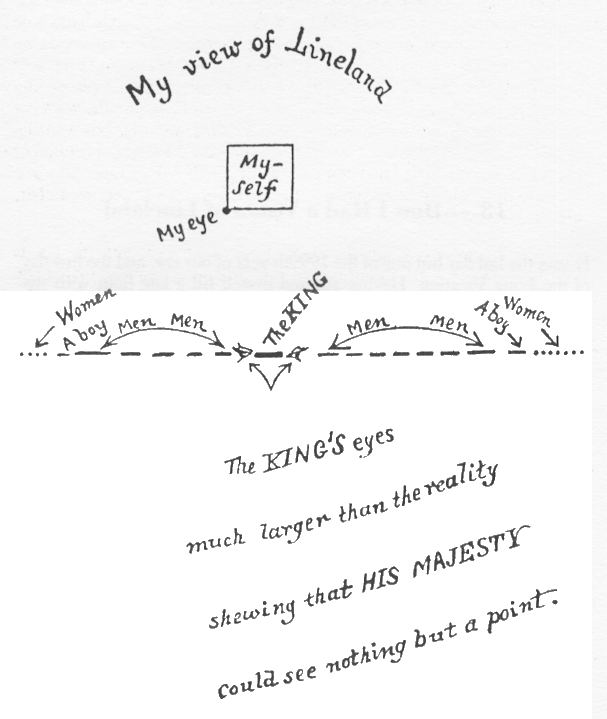
\includegraphics[trim=0mm 0mm 0mm 0mm,width=\linewidth]{fig6}

It seemed that this poor ignorant Monarch --- as he called himself --- was
persuaded that the Straight Line which he called his Kingdom, and in which he
passed his existence, constituted the whole of the world, and indeed the whole
of Space. Not being able either to move or to see, save in his Straight Line,
he had no conception of anything out of it. Though he had heard my voice when
I first addressed him, the sounds had come to him in a manner so contrary to
his experience that he had made no answer, ``seeing no man,'' as he expressed
it, ``and hearing a voice as it were from my own intestines.'' Until the moment
when I placed my mouth in his World, he had neither seen me, nor heard
anything except confused sounds beating against, what I called his side, but
what he called his \emph{inside} or \emph{stomach}; nor had he even now the least conception
of the region from which I had come. Outside his World, or Line, all was a
blank to him; nay, not even a blank, for a blank implies Space; say, rather,
all was non-existent.

His subjects --- of whom the small Lines were men and the Points Women --- were
all alike confined in motion and eyesight to that single Straight Line, which
was their World. It need scarcely be added that the whole of their horizon was
limited to a Point; nor could any one ever see anything but a Point. Man,
woman, child, thing --- each as a Point to the eye of a Linelander. Only by the
sound of the voice could sex or age be distinguished. Moreover, as each
individual occupied the whole of the narrow path, so to speak, which
constituted his Universe, and no one could move to the right or left to make
way for passers by, it followed that no Linelander could ever pass another.
Once neighbours, always neighbours. Neighbourhood with them was like marriage
with us. Neighbours remained neighbours till death did them part.

Such a life, with all vision limited to a Point, and all motion to a Straight
Line, seemed to me inexpressibly dreary; and I was surprised to note that
vivacity and cheerfulness of the King. Wondering whether it was possible, amid
circumstances so unfavourable to domestic relations, to enjoy the pleasures of
conjugal union, I hesitated for some time to question his Royal Highness on so
delicate a subject; but at last I plunged into it by abruptly inquiring as to
the health of his family. ``My wives and children,'' he replied, ``are well and
happy.''

Staggered at this answer --- for in the immediate proximity of the Monarch (as I
had noted in my dream before I entered Lineland) there were none but Men --- I
ventured to reply, ``Pardon me, but I cannot imagine how your Royal Highness
can at any time either See or approach their Majesties, when there at least
half a dozen intervening individuals, whom you can neither see through, nor
pass by? Is it possible that in Lineland proximity is not necessary for
marriage and for the generation of children?''

``How can you ask so absurd a question?'' replied the Monarch. ``If it were
indeed as you suggest, the Universe would soon be depopulated. No, no;
neighbourhood is needless for the union of hearts; and the birth of children
is too important a matter to have been allowed to depend upon such an accident
as proximity. You cannot be ignorant of this. Yet since you are pleased to
affect ignorance, I will instruct you as if you were the veriest baby in
Lineland. Know, then, that marriages are consummated by means of the faculty
of sound and the sense of hearing.

``You are of course aware that every Man has two mouths or voices --- as well as
two eyes --- a bass at one and a tenor at the other of his extremities. I should
not mention this, but that I have been unable to distinguish your tenor in the
course of our conversation.'' I replied that I had but one voice, and that I
had not been aware that his Royal Highness had two. ``That confirms by
impression,'' said the King, ``that you are not a Man, but a feminine
Monstrosity with a bass voice, and an utterly uneducated ear. But to continue.

``Nature having herself ordained that every Man should wed two wives ---'' ``Why
two?'' asked I. ``You carry your affected simplicity too far,'' he cried. ``How
can there be a completely harmonious union without the combination of the Four
in One, viz.\@ the Bass and Tenor of the Man and the Soprano and Contralto of
the two Women?'' ``But supposing,'' said I, ``that a man should prefer one wife or
three?'' ``It is impossible,'' he said; ``it is as inconceivable as that two and
one should make five, or that the human eye should see a Straight Line.'' I
would have interrupted him; but he proceeded as follows:

``Once in the middle of each week a Law of Nature compels us to move to and fro
with a rhythmic motion of more than usual violence, which continues for the
time you would take to count a hundred and one. In the midst of this choral
dance, at the fifty-first pulsation, the inhabitants of the Universe pause in
full career, and each individual sends forth his richest, fullest, sweetest
strain. It is in this decisive moment that all our marriages are made. So
exquisite is the adaptation of Bass and Treble, of Tenor to Contralto, that
oftentimes the Loved Ones, though twenty thousand leagues away, recognize at
once the responsive note of their destined Lover; and, penetrating the paltry
obstacles of distance, Love unites the three. The marriage in that instance
consummated results in a threefold Male and Female offspring which takes its
place in Lineland.''

``What! Always threefold?'' said I. ``Must one wife then always have twins?''

``Bass-voice Monstrosity! yes,'' replied the King. ``How else could the balance
of the Sexes be maintained, if two girls were not born for every boy? Would
you ignore the very Alphabet of Nature?'' He ceased, speechless for fury; and
some time elapsed before I could induce him to resume his narrative.

``You will not, of course, suppose that every bachelor among us finds his mates
at the first wooing in this universal Marriage Chorus. On the contrary, the
process is by most of us many times repeated. Few are the hearts whose happy
lot is at once to recognize in each other's voice the partner intended for
them by Providence, and to fly into a reciprocal and perfectly harmonious
embrace. With most of us the courtship is of long duration. The Wooer's voices
may perhaps accord with one of the future wives, but not with both; or not, at
first, with either; or the Soprano and Contralto may not quite harmonize. In
such cases Nature has provided that every weekly Chorus shall bring the three
Lovers into closer harmony. Each trial of voice, each fresh discovery of
discord, almost imperceptibly induces the less perfect to modify his or her
vocal utterance so as to approximate to the more perfect. And after many
trials and many approximations, the result is at last achieved. There comes a
day at last when, while the wonted Marriage Chorus goes forth from universal
Lineland, the three far-off Lovers suddenly find themselves in exact harmony,
and, before they are aware, the wedded Triplet is rapt vocally into a
duplicate embrace; and Nature rejoices over one more marriage and over three
more births.''


\chapter{How I vainly tried to explain the nature of Flatland}


Thinking that it was time to bring down the Monarch from his raptures to the
level of common sense, I determined to endeavour to open up to him some
glimpses of the truth, that is to say of the nature of things in Flatland. So
I began thus: ``How does your Royal Highness distinguish the shapes and
positions of his subjects? I for my part noticed by the sense of sight, before
I entered your Kingdom, that some of your people are lines and others Points;
and that some of the lines are larger ---'' ``You speak of an impossibility,''
interrupted the King; ``you must have seen a vision; for to detect the
difference between a Line and a Point by the sense of sight is, as every one
knows, in the nature of things, impossible; but it can be detected by the
sense of hearing, and by the same means my shape can be exactly ascertained.
Behold me --- I am a Line, the longest in Lineland, over six inches of Space ---''
``Of Length,'' I ventured to suggest. ``Fool,'' said he, ``Space is Length.
Interrupt me again, and I have done.''

I apologized; but he continued scornfully, ``Since you are impervious to
argument, you shall hear with your ears how by means of my two voices I reveal
my shape to my Wives, who are at this moment six thousand miles seventy yards
two feet eight inches away, the one to the North, the other to the South.
Listen, I call to them.''

He chirruped, and then complacently continued: ``My wives at this moment
receiving the sound of one of my voice, closely followed by the other, and
perceiving that the latter reaches them after an interval in which sound can
traverse 6.457 inches, infer that one of my mouths is 6.457 inches further
from them than the other, and accordingly know my shape to be 6.457 inches.
But you will of course understand that my wives do not make this calculation
every time they hear my two voices. They made it, once for all, before we were
married. But they \emph{could} make it at any time. And in the same way I can
estimate the shape of any of my Male subjects by the sense of sound.''

``But how,'' said I, ``if a Man feigns a Woman's voice with one of his two
voices, or so disguises his Southern voice that it cannot be recognized as the
echo of the Northern? May not such deceptions cause great inconvenience? And
have you no means of checking frauds of this kind by commanding your
neighbouring subjects to feel one another?'' This of course was a very stupid
question, for feeling could not have answered the purpose; but I asked with
the view of irritating the Monarch, and I succeeded perfectly.

``What!'' cried he in horror, ``explain your meaning.'' ``Feel, touch, come into
contact,'' I replied.. ``If you mean by \emph{feeling},`` said the King, ``approaching so
close as to leave no space between two individuals, know, Stranger, that this
offence is punishable in my dominions by death. And the reason is obvious. The
frail form of a Woman, being liable to be shattered by such an approximation,
must be preserved by the State; but since Women cannot be distinguished by the
sense of sight from Men, the Law ordains universally that neither Man nor
Woman shall be approached so closely as to destroy the interval between the
approximator and the approximated.

``And indeed what possible purpose would be served by this illegal and
unnatural excess of approximation which you call \emph{touching}, when all the ends
of so brutal and course a process are attained at once more easily and more
exactly by the sense of hearing? As to your suggested danger of deception, it
is non-existent: for the Voice, being the essence of one's Being, cannot be
thus changed at will. But come, suppose that I had the power of passing
through solid things, so that I could penetrate my subjects, one after
another, even to the number of a billion, verifying the size and distance of
each by the sense of \emph{feeling}: How much time and energy would be wasted in this
clumsy and inaccurate method! Whereas now, in one moment of audition, I take
as it were the census and statistics, local, corporeal, mental and spiritual,
of every living being in Lineland. Hark, only hark!''

So saying he paused and listened, as if in an ecstasy, to a sound which seemed
to me no better than a tiny chirping from an innumerable multitude of
lilliputian grasshoppers.

``Truly,'' replied I, ``your sense of hearing serves you in good stead, and fills
up many of your deficiencies. But permit me to point out that your life in
Lineland must be deplorably dull. To see nothing but a Point! Not even to be
able to contemplate a Straight Line! Nay, not even to know what a Straight
Line is! To see, yet to be cut off from those Linear prospects which are
vouchsafed to us in Flatland! Better surely to have no sense of sight at all
than to see so little! I grant you I have not your discriminative faculty of
hearing; for the concert of all Lineland which gives you such intense
pleasure, is to me no better than a multitudinous twittering or chirping. But
at least I can discern, by sight, a Line from a Point. And let me prove it.
Just before I came into your kingdom, I saw you dancing from left to right,
and then from right to left, with Seven Men and a Woman in your immediate
proximity on the left, and eight Men and two Women on your right. Is not this
correct?''

``It is correct,'' said the King, ``so far as the numbers and sexes are
concerned, though I know not what you mean by `right' and `left.' But I deny
that you saw these things. For how could you see the Line, that is to say the
inside, of any Man? But you must have heard these things, and then dreamed
that you saw them. And let me ask what you mean by those words `left' and
`right'. I suppose it is your way of saying Northward and Southward.''

``Not so,'' replied I; ``besides your motion of Northward and Southward, there is
another motion which I call from right to left.''

\emph{King}. Exhibit to me, if you please, this motion from left to right.

\emph{I}. Nay, that I cannot do, unless you could step out of your Line altogether.

\emph{King}. Out of my Line? Do you mean out of the world? Out of Space?

\emph{I}. Well, yes. Out of \emph{your} world. Out of \emph{your} Space. For your Space is not the
true Space. True Space is a Plane; but your Space is only a Line.

\emph{King}. If you cannot indicate this motion from left to right by yourself moving
in it, then I beg you to describe it to me in words.

\emph{I}. If you cannot tell your right side from your left, I fear that no words of
mine can make my meaning clearer to you. But surely you cannot be ignorant of
so simple a distinction.

\emph{King}. I do not in the least understand you.

\emph{I}. Alas! How shall I make it clear? When you move straight on, does it not
sometimes occur to you that you \emph{could} move in some other way, turning your eye
round so as to look in the direction towards which your side is now fronting?
In other words, instead of always moving in the direction of one of your
extremities, do you never feel a desire to move in the direction, so to speak,
of your side?

\emph{King}. Never. And what do you mean? How can a man's inside ``front'' in any
direction? Or how can a man move in the direction of his inside?

\emph{I}. Well then, since words cannot explain the matter, I will try deeds, and
will move gradually out of Lineland in the direction which I desire to
indicate to you.

At the word I began to move my body out of Lineland. As long as any part of me
remained in his dominion and in his view, the King kept exclaiming, ``I see
you, I see you still; you are not moving.'' But when I had at last moved myself
out of his Line, he cried in his shrillest voice, ``She is vanished; she is
dead.'' ``I am not dead,'' replied I; ``I am simply out of Lineland, that is to
say, out of the Straight Line which you call Space, and in the true Space,
where I can see things as they are. And at this moment I can see your Line, or
side --- or inside as you are pleased to call it; and I can see also the Men and
Women on the North and South of you, whom I will now enumerate, describing
their order, their size, and the interval between each.''

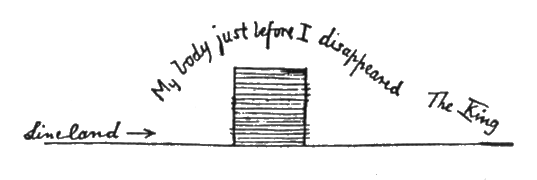
\includegraphics[trim=0mm 0mm 0mm 0mm,width=\linewidth]{fig7}

When I had done this at great length, I cried triumphantly, ``Does that at last
convince you?'' And, with that, I once more entered Lineland, taking up the
same position as before.

But the Monarch replied, ``If you were a Man of sense --- though, as you appear
to have only one voice I have little doubt you are not a Man but a Woman ---
but, if you had a particle of sense, you would listen to reason. You ask me to
believe that there is another Line besides that which my senses indicate, and
another motion besides that of which I am daily conscious. I, in return, ask
you to describe in words or indicate by motion that other Line of which you
speak. Instead of moving, you merely exercise some magic art of vanishing and
returning to sight; and instead of any lucid description of your new World,
you simply tell me the numbers and sizes of some forty of my retinue, facts
known to any child in my capital. Can anything be more irrational or
audacious? Acknowledge your folly or depart from my dominions.''

Furious at his perversity, and especially indignant that he professed to be
ignorant of my sex, I retorted in no measured terms, ``Besotted Being! You
think yourself the perfection of existence, while you are in reality the most
imperfect and imbecile. You profess to see, whereas you see nothing but a
Point! You plume yourself on inferring the existence of a Straight Line; but I
\emph{can see} Straight Lines, and infer the existence of Angles, Triangles, Squares,
Pentagons, Hexagons, and even Circles. Why waste more words? Suffice it that I
am the completion of your incomplete self. You are a Line, but I am a Line of
Lines called in my country a Square: and even I, infinitely superior though I
am to you, am of little account among the great nobles of Flatland, whence I
have come to visit you, in the hope of enlightening your ignorance.''

Hearing these words the King advanced towards me with a menacing cry as if to
pierce me through the diagonal; and in that same movement there arose from
myriads of his subjects a multitudinous war-cry, increasing in vehemence till
at last methought it rivalled the roar of an army of a hundred thousand
Isosceles, and the artillery of a thousand Pentagons. Spell-bound and
motionless, I could neither speak nor move to avert the impending destruction;
and still the noise grew louder, and the King came closer, when I awoke to
find the breakfast-bell recalling me to the realities of Flatland.


\chapter{Concerning a Stranger from Spaceland}


From dreams I proceed to facts.

It was the last day of our 1999th year of our era. The patterning of the rain
had long ago announced nightfall; and I was sitting~\footnote{When I say
``sitting,'' of course I do not mean any change of attitude such as you in
Spaceland signify by that word; for as we have no feet, we can no more ``sit''
nor ``stand'' (in your sense of the word) than one of your soles or flounders.

Nevertheless, we perfectly well recognize the different mental states of
volition implied by ``lying,'' ``sitting,'' and ``standing,'' which are to some
extent indicated to a beholder by a slight increase of lustre corresponding to
the increase of volition.

But on this, and a thousand other kindred subjects, time forbids me to dwell.}
in the company of my wife, musing on the events of the past and the prospects
of the coming year, the coming century, the coming Millennium.

My four Sons and two orphan Grandchildren had retired to their several
apartments; and my wife alone remained with me to see the old Millennium out
and the new one in.

I was rapt in thought, pondering in my mind some words that had casually
issued from the mouth of my youngest Grandson, a most promising young Hexagon
of unusual brilliancy and perfect angularity. His uncles and I had been giving
him his usual practical lesson in Sight Recognition, turning ourselves upon
our centres, now rapidly, now more slowly, and questioning him as to our
positions; and his answers had been so satisfactory that I had been induced to
reward him by giving him a few hints on Arithmetic, as applied to Geometry.

Taking nine Squares, each an inch every way, I had put them together so as to
make one large Square, with a side of three inches, and I had hence proved to
my little Grandson that --- though it was impossible for us to see the inside of
the Square --- yet we might ascertain the number of square inches in a Square by
simply squaring the number of inches in the side: ``and thus,'' said I, ``we know
that three-to-the-second, or nine, represents the number of square inches in a
Square whose side is three inches long.''

The little Hexagon meditated on this a while and then said to me; ``But you
have been teaching me to raise numbers to the third power: I suppose
three-to-the-third must mean something in Geometry; what does it mean?''
``Nothing at all,'' replied I, ``not at least in Geometry; for Geometry has only
Two Dimensions.'' And then I began to shew the boy how a Point by moving
through a length of three inches makes a Line of three inches, which may be
represented by three; and how a Line of three inches, moving parallel to
itself through a length of three inches, makes a Square of three inches every
way, which may be represented by three-to-the-second.

Upon this, my Grandson, again returning to his former suggestion, took me up
rather suddenly and exclaimed, ``Well, then, if a Point by moving three inches,
makes a Line of three inches represented by three; and if a straight Line of
three inches, moving parallel to itself, makes a Square of three inches every
way, represented by three-to-the-second; it must be that a Square of three
inches every way, moving somehow parallel to itself (but I don't see how) must
make Something else (but I don't see what) of three inches every way --- and
this must be represented by three-to-the-third.''

``Go to bed,'' said I, a little ruffled by this interruption: ``if you would talk
less nonsense, you would remember more sense.''

So my Grandson had disappeared in disgrace; and there I sat by my Wife's side,
endeavouring to form a retrospect of the year 1999 and of the possibilities of
the year 2000; but not quite able to shake of the thoughts suggested by the
prattle of my bright little Hexagon. Only a few sands now remained in the
half-hour glass. Rousing myself from my reverie I turned the glass Northward
for the last time in the old Millennium; and in the act, I exclaimed aloud,
``The boy is a fool.''

Straightway I became conscious of a Presence in the room, and a chilling
breath thrilled through my very being. ``He is no such thing,'' cried my Wife,
``and you are breaking the Commandments in thus dishonouring your own
Grandson.'' But I took no notice of her. Looking around in every direction I
could see nothing; yet still I \emph{felt} a Presence, and shivered as the cold
whisper came again. I started up. ``What is the matter?'' said my Wife, ``there
is no draught; what are you looking for? There is nothing.'' There was nothing;
and I resumed my seat, again exclaiming, ``The boy is a fool, I say;
three-to-the-third can have no meaning in Geometry.'' At once there came a
distinctly audible reply, ``The boy is not a fool; and three-to-the-third has
an obvious Geometrical meaning.''

My Wife as well as myself heard the words, although she did not understand
their meaning, and both of us sprang forward in the direction of the sound.
What was our horror when we saw before us a Figure! At the first glance it
appeared to be a Woman, seen sideways; but a moment's observation shewed me
that the extremities passed into dimness too rapidly to represent one of the
Female Sex; and I should have thought it a Circle, only that it seemed to
change its size in a manner impossible for a Circle or for any regular Figure
of which I had had experience.

But my Wife had not my experience, nor the coolness necessary to note these
characteristics. With the usual hastiness and unreasoning jealousy of her Sex,
she flew at once to the conclusion that a Woman had entered the house through
some small aperture. ``How comes this person here?'' she exclaimed, ``you
promised me, my dear, that there should be no ventilators in our new house.''
``Nor are they any,'' said I; ``but what makes you think that the stranger is a
Woman? I see by my power of Sight Recognition ---'' ``Oh, I have no patience with
your Sight Recognition,'' replied she, ```Feeling is believing' and `A Straight
Line to the touch is worth a Circle to the sight'\, '' --- two Proverbs, very common
with the Frailer Sex in Flatland.

``Well,'' said I, for I was afraid of irritating her, ``if it must be so, demand
an introduction.'' Assuming her most gracious manner, my Wife advanced towards
the Stranger, ``Permit me, Madam to feel and be felt by ---'' then, suddenly
recoiling, ``Oh! it is not a Woman, and there are no angles either, not a trace
of one. Can it be that I have so misbehaved to a perfect Circle?''

``I am indeed, in a certain sense a Circle,'' replied the Voice, ``and a more
perfect Circle than any in Flatland; but to speak more accurately, I am many
Circles in one.'' Then he added more mildly, ``I have a message, dear Madam, to
your husband, which I must not deliver in your presence; and, if you would
suffer us to retire for a few minutes ---'' But my wife would not listen to the
proposal that our august Visitor should so incommode himself, and assuring the
Circle that the hour of her own retirement had long passed, with many
reiterated apologies for her recent indiscretion, she at last retreated to her
apartment.

I glanced at the half-hour glass. The last sands had fallen. The third
Millennium had begun.


\chapter{How the Stranger vainly endeavoured to reveal to me in words the mysteries of Spaceland}


As soon as the sound of the Peace-cry of my departing Wife had died away, I
began to approach the Stranger with the intention of taking a nearer view and
of bidding him be seated: but his appearance struck me dumb and motionless
with astonishment. Without the slightest symptoms of angularity he
nevertheless varied every instant with graduations of size and brightness
scarcely possible for any Figure within the scope of my experience. The
thought flashed across me that I might have before me a burglar or cut-throat,
some monstrous Irregular Isosceles, who, by feigning the voice of a Circle,
had obtained admission somehow into the house, and was now preparing to stab
me with his acute angle.

In a sitting-room, the absence of Fog (and the season happened to be
remarkably dry), made it difficult for me to trust to Sight Recognition,
especially at the short distance at which I was standing. Desperate with fear,
I rushed forward with an unceremonious, ``You must permit me, Sir ---'' and felt
him. My Wife was right. There was not the trace of an angle, not the slightest
roughness or inequality: never in my life had I met with a more perfect
Circle. He remained motionless while I walked around him, beginning from his
eye and returning to it again. Circular he was throughout, a perfectly
satisfactory Circle; there could not be a doubt of it. Then followed a
dialogue, which I will endeavour to set down as near as I can recollect it,
omitting only some of my profuse apologies --- for I was covered with shame and
humiliation that I, a Square, should have been guilty of the impertinence of
feeling a Circle. It was commenced by the Stranger with some impatience at the
lengthiness of my introductory process.

\emph{STRANGER}. Have you felt me enough by this time? Are you not introduced to me
yet?

\emph{I}. Most illustrious Sir, excuse my awkwardness, which arises not from
ignorance of the usages of polite society, but from a little surprise and
nervousness, consequent on this somewhat unexpected visit. And I beseech you
to reveal my indiscretion to no one, and especially not to my Wife. But before
your Lordship enters into further communications, would he deign to satisfy
the curiosity of one who would gladly know whence his visitor came?

\emph{STRANGER}. From Space, from Space, Sir: whence else?

\emph{I}. Pardon me, my Lord, but is not your Lordship already in Space, your
Lordship and his humble servant, even at this moment?

\emph{STRANGER}. Pooh! what do you know of Space? Define Space.

\emph{I}. Space, my Lord, is height and breadth indefinitely prolonged.

\emph{STRANGER}. Exactly: you see you do not even know what Space is. You think it is
of Two Dimensions only; but I have come to announce to you a Third --- height,
breadth, and length.

\emph{I}. Your Lordship is pleased to be merry. We also speak of length and height,
or breadth and thickness, thus denoting Two Dimensions by four names.

\emph{STRANGER}. But I mean not only three names, but Three Dimensions.

\emph{I}. Would your Lordship indicate or explain to me in what direction is the
Third Dimension, unknown to me?

\emph{STRANGER}. I came from it. It is up above and down below.

\emph{I}. My Lord means seemingly that it is Northward and Southward.

\emph{STRANGER}. I mean nothing of the kind. I mean a direction in which you cannot
look, because you have no eye in your side.

\emph{I}. Pardon me, my Lord, a moment's inspection will convince your Lordship that
I have a perfectly luminary at the juncture of my two sides.

\emph{STRANGER}: Yes: but in order to see into Space you ought to have an eye, not on
your Perimeter, but on your side, that is, on what you would probably call
your inside; but we in Spaceland should call it your side.

\emph{I}. An eye in my inside! An eye in my stomach! Your Lordship jests.

\emph{STRANGER}. I am in no jesting humour. I tell you that I come from Space, or,
since you will not understand what Space means, from the Land of Three
Dimensions whence I but lately looked down upon your Plane which you call
Space forsooth. From that position of advantage I discerned all that you speak
of as \emph{solid} (by which you mean ``enclosed on four sides''), your houses, your
churches, your very chests and safes, yes even your insides and stomachs, all
lying open and exposed to my view.

\emph{I}. Such assertions are easily made, my Lord.

\emph{STRANGER}. But not easily proved, you mean. But I mean to prove mine.

When I descended here, I saw your four Sons, the Pentagons, each in his
apartment, and your two Grandsons the Hexagons; I saw your youngest Hexagon
remain a while with you and then retire to his room, leaving you and your Wife
alone. I saw your Isosceles servants, three in number, in the kitchen at
supper, and the little Page in the scullery. Then I came here, and how do you
think I came?

\emph{I}. Through the roof, I suppose.

\emph{STRANGER}. Not so. Your roof, as you know very well, has been recently
repaired, and has no aperture by which even a Woman could penetrate. I tell
you I come from Space. Are you not convinced by what I have told you of your
children and household?

\emph{I}. Your Lordship must be aware that such facts touching the belongings of his
humble servant might be easily ascertained by any one of the neighbourhood
possessing your Lordship's ample means of information.

\emph{STRANGER}. (\emph{To himself}.) What must I do? Stay; one more argument suggests
itself to me. When you see a Straight Line --- your wife, for example --- how many
Dimensions do you attribute to her?

\emph{I}. Your Lordship would treat me as if I were one of the vulgar who, being
ignorant of Mathematics, suppose that a Woman is really a Straight Line, and
only of One Dimension. No, no, my Lord; we Squares are better advised, and are
as well aware of your Lordship that a Woman, though popularly called a
Straight Line, is, really and scientifically, a very thin Parallelogram,
possessing Two Dimensions, like the rest of us, viz., length and breadth (or
thickness).

\emph{STRANGER}. But the very fact that a Line is visible implies that it possesses
yet another Dimension.

\emph{I}. My Lord, I have just acknowledge that a Woman is broad as well as long. We
see her length, we infer her breadth; which, though very slight, is capable of
measurement.

\emph{STRANGER}. You do not understand me. I mean that when you see a Woman, you
ought --- besides inferring her breadth --- to see her length, and to \emph{see} what we
call her \emph{height}; although the last Dimension is infinitesimal in your country.
If a Line were mere length without ``height,'' it would cease to occupy Space
and would become invisible. Surely you must recognize this?

\emph{I}. I must indeed confess that I do not in the least understand your Lordship.
When we in Flatland see a Line, we see length and \emph{brightness}. If the
brightness disappears, the Line is extinguished, and, as you say, ceases to
occupy Space. But am I to suppose that your Lordship gives the brightness the
title of a Dimension, and that what we call ``bright'' you call ``high''?

\emph{STRANGER}. No, indeed. By ``height'' I mean a Dimension like your length: only,
with you, ``height'' is not so easily perceptible, being extremely small.

\emph{I}. My Lord, your assertion is easily put to the test. You say I have a Third
Dimension, which you call ``height.'' Now, Dimension implies direction and
measurement. Do but measure my ``height,'' or merely indicate to me the
direction in which my ``height'' extends, and I will become your convert.
Otherwise, your Lordship's own understanding must hold me excused.

\emph{STRANGER}. (\emph{To himself}.) I can do neither. How shall I convince him? Surely a
plain statement of facts followed by ocular demonstration ought to suffice. ---
Now, Sir; listen to me.

You are living on a Plane. What you style Flatland is the vast level surface
of what I may call a fluid, or in, the top of which you and your countrymen
move about, without rising above or falling below it.

I am not a plane Figure, but a Solid. You call me a Circle; but in reality I
am not a Circle, but an infinite number of Circles, of size varying from a
Point to a Circle of thirteen inches in diameter, one placed on the top of the
other. When I cut through your plane as I am now doing, I make in your plane a
section which you, very rightly, call a Circle. For even a Sphere --- which is
my proper name in my own country --- if he manifest himself at all to an
inhabitant of Flatland --- must needs manifest himself as a Circle.

Do you not remember --- for I, who see all things, discerned last night the
phantasmal vision of Lineland written upon your brain --- do you not remember, I
say, how when you entered the realm of Lineland, you were compelled to
manifest yourself to the King, not as a Square, but as a Line, because that
Linear Realm had not Dimensions enough to represent the whole of you, but only
a slice or section of you? In precisely the same way, your country of Two
Dimensions is not spacious enough to represent me, a being of Three, but can
only exhibit a slice or section of me, which is what you call a Circle.

The diminished brightness of your eye indicates incredulity. But now prepare
to receive proof positive of the truth of my assertions. You cannot indeed see
more than one of my sections, or Circles, at a time; for you have no power to
raise your eye out of the plane of Flatland; but you can at least see that, as
I rise in Space, so my sections become smaller. See now, I will rise; and the
effect upon your eye will be that my Circle will become smaller and smaller
till it dwindles to a point and finally vanishes.

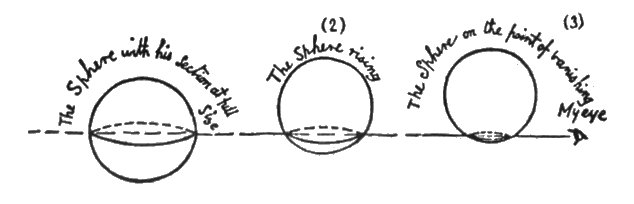
\includegraphics[trim=25mm 0mm 0mm 0mm,width=\linewidth]{fig8}

There was no ``rising'' that I could see; but he diminished and finally
vanished. I winked once or twice to make sure that I was not dreaming. But it
was no dream. For from the depths of nowhere came forth a hollow voice --- close
to my heart it seemed --- ``Am I quite gone? Are you convinced now? Well, now I
will gradually return to Flatland and you shall see my section become larger
and larger.''

Every reader in Spaceland will easily understand that my mysterious Guest was
speaking the language of truth and even of simplicity. But to me, proficient
though I was in Flatland Mathematics, it was by no means a simple matter. The
rough diagram given above will make it clear to any Spaceland child that the
Sphere, ascending in the three positions indicated there, must needs have
manifested himself to me, or to any Flatlander, as a Circle, at first of full
size, then small, and at last very small indeed, approaching to a Point. But
to me, although I saw the facts before me, the causes were as dark as ever.
All that I could comprehend was, that the Circle had made himself smaller and
vanished, and that he had now re-appeared and was rapidly making himself
larger.

When he regained his original size, he heaved a deep sigh; for he perceived by
my silence that I had altogether failed to comprehend him. And indeed I was
now inclining to the belief that he must be no Circle at all, but some
extremely clever juggler; or else that the old wives' tales were true, and
that after all there were such people as Enchanters and Magicians.

After a long pause he muttered to himself, ``One resource alone remains, if I
am not to resort to action. I must try the method of Analogy.'' Then followed a
still longer silence, after which he continued our dialogue.

\emph{SPHERE}. Tell me, Mr. Mathematician; if a Point moves Northward, and leaves a
luminous wake, what name would you give to the wake?

\emph{I}. A straight Line.

\emph{SPHERE}. And a straight Line has how many extremities?

\emph{I}. Two.

\emph{SPHERE}. Now conceive the Northward straight Line moving parallel to itself,
East and West, so that every point in it leaves behind it the wake of a
straight Line. What name will you give to the Figure thereby formed? We will
suppose that it moves through a distance equal to the original straight line.
--- What name, I say?

\emph{I}. A square.

\emph{SPHERE}. And how many sides has a Square? How many angles?

\emph{I}. Four sides and four angles.

\emph{SPHERE}. Now stretch your imagination a little, and conceive a Square in
Flatland, moving parallel to itself upward.

\emph{I}. What? Northward?

\emph{SPHERE}. No, not Northward; upward; out of Flatland altogether.

If it moved Northward, the Southern points in the Square would have to move
through the positions previously occupied by the Northern points. But that is
not my meaning.

I mean that every Point in you --- for you are a Square and will serve the
purpose of my illustration --- every Point in you, that is to say in what you
call your inside, is to pass upwards through Space in such a way that no Point
shall pass through the position previously occupied by any other Point; but
each Point shall describe a straight Line of its own. This is all in
accordance with Analogy; surely it must be clear to you.

Restraining my impatience --- for I was now under a strong temptation to rush
blindly at my Visitor and to precipitate him into Space, or out of Flatland,
anywhere, so that I could get rid of him --- I replied: ---

``And what may be the nature of the Figure which I am to shape out by this
motion which you are pleased to denote by the word `upward'? I presume it is
describable in the language of Flatland.''

\emph{SPHERE}. Oh, certainly. It is all plain and simple, and in strict accordance
with Analogy --- only, by the way, you must not speak of the result as being a
Figure, but as a Solid. But I will describe it to you. Or rather not I, but
Analogy.

We began with a single Point, which of course --- being itself a Point --- has
only \emph{one} terminal Point.

One Point produces a Line with \emph{two} terminal Points.

One Line produces a Square with \emph{four} terminal Points.

Now you can give yourself the answer to your own question: 1, 2, 4, are
evidently in Geometrical Progression. What is the next number?

\emph{I}. Eight.

\emph{SPHERE}. Exactly. The one Square produces a
\emph{Something-which-you-do-not-as-yet-know-a-name-for-but-which-we-call-a-Cube}
with \emph{eight} terminal Points. Now are you convinced?

\emph{I}. And has this Creature sides, as well as Angles or what you call ``terminal
Points''?

\emph{SPHERE}. Of course; and all according to Analogy. But, by the way, not what \emph{you}
call sides, but what \emph{we} call sides. You would call them \emph{solids}.

\emph{I}. And how many solids or sides will appertain to this Being whom I am to
generate by the motion of my inside in an ``upward'' direction, and whom you
call a Cube?

\emph{SPHERE}. How can you ask? And you a mathematician! The side of anything is
always, if I may so say, one Dimension behind the thing. Consequently, as
there is no Dimension behind a Point, a Point has 0 sides; a Line, if I may so
say, has 2 sides (for the points of a Line may be called by courtesy, its
sides); a Square has 4 sides; 0, 2, 4; what Progression do you call that?

\emph{I}. Arithmetical.

\emph{SPHERE}. And what is the next number?

\emph{I}. Six.

\emph{SPHERE}. Exactly. Then you see you have answered your own question. The Cube
which you will generate will be bounded by six sides, that is to say, six of
your insides. You see it all now, eh?

``Monster,'' I shrieked, ``be thou juggler, enchanter, dream, or devil, no more
will I endure thy mockeries. Either thou or I must perish.'' And saying these
words I precipitated myself upon him.


\chapter{How the Sphere, having in vain tried words, resorted to deeds}


It was in vain. I brought my hardest right angle into violent collision with
the Stranger, pressing on him with a force sufficient to have destroyed any
ordinary Circle: but I could feel him slowly and unarrestably slipping from my
contact; not edging to the right nor to the left, but moving somehow out of
the world, and vanishing into nothing. Soon there was a blank. But still I
heard the Intruder's voice.

\emph{SPHERE}. Why will you refuse to listen to reason? I had hoped to find in you ---
as being a man of sense and an accomplished mathematician --- a fit apostle for
the Gospel of the Three Dimensions, which I am allowed to preach once only in
a thousand years: but now I know not how to convince you. Stay, I have it.
Deeds, and not words, shall proclaim the truth. Listen, my friend.

I have told you I can see from my position in Space the inside of all things
that you consider closed. For example, I see in yonder cupboard near which you
are standing, several of what you call boxes (but like everything else in
Flatland, they have no tops or bottom) full of money; I see also two tablets
of accounts. I am about to descend into that cupboard and to bring you one of
those tablets. I saw you lock the cupboard half an hour ago, and I know you
have the key in your possession. But I descend from Space; the doors, you see,
remain unmoved. Now I am in the cupboard and am taking the tablet. Now I have
it. Now I ascent with it.

I rushed to the closet and dashed the door open. One of the tablets was gone.
With a mocking laugh, the Stranger appeared in the other corner of the room,
and at the same time the tablet appeared upon the floor. I took it up. There
could be no doubt --- it was the missing tablet.

I groaned with horror, doubting whether I was not out of my sense; but the
Stranger continued: ``Surely you must now see that my explanation, and no
other, suits the phenomena. What you call Solid things are really superficial;
what you call Space is really nothing but a great Plane. I am in Space, and
look down upon the insides of the things of which you only see the outsides.
You could leave the Plane yourself, if you could but summon up the necessary
volition. A slight upward or downward motion would enable you to see all that
I can see.

``The higher I mount, and the further I go from your Plane, the more I can see,
though of course I see it on a smaller scale. For example, I am ascending; now
I can see your neighbour the Hexagon and his family in their several
apartments; now I see the inside of the Theatre, ten doors off, from which the
audience is only just departing; and on the other side a Circle in his study,
sitting at his books. Now I shall come back to you. And, as a crowning proof,
what do you say to my giving you a touch, just the least touch, in your
stomach? It will not seriously injure you, and the slight pain you may suffer
cannot be compared with the mental benefit you will receive.''

Before I could utter a word of remonstrance, I felt a shooting pain in my
inside, and a demoniacal laugh seemed to issue from within me. A moment
afterwards the sharp agony had ceased, leaving nothing but a dull ache behind,
and the Stranger began to reappear, saying, as he gradually increased in size,
``There, I have not hurt you much, have I? If you are not convinced now, I
don't know what will convince you. What say you?''

My resolution was taken. It seemed intolerable that I should endure existence
subject to the arbitrary visitations of a Magician who could thus play tricks
with one's very stomach. If only I could in any way manage to pin him against
the wall till help came!

Once more I dashed my hardest angle against him, at the same time alarming the
whole household by my cries for aid. I believe, at the moment of my onset, the
Stranger had sunk below our Plane, and really found difficulty in rising. In
any case he remained motionless, while I, hearing, as I thought, the sound of
some help approaching, pressed against him with redoubled vigor, and continued
to shout for assistance.

A convulsive shudder ran through the Sphere. ``This must not be,'' I thought I
heard him say: ``either he must listen to reason, or I must have recourse to
the last resource of civilization.'' Then, addressing me in a louder tone, he
hurriedly exclaimed, ``Listen: no stranger must witness what you have
witnessed. Send your Wife back at once, before she enters the apartment. The
Gospel of Three Dimensions must not be thus frustrated. Not thus must the
fruits of one thousand years of waiting be thrown away. I hear her coming.
Back! back! Away from me, or you must go with me --- wither you know not --- into
the Land of Three Dimensions!''

``Fool! Madman! Irregular!'' I exclaimed; ``never will I release thee; thou shalt
pay the penalty of thine impostures.''

``Ha! Is it come to this?'' thundered the Stranger: ``then meet your fate: out of
your Plane you go. Once, twice, thrice! 'Tis done!''


\chapter{How I came to Spaceland, and what I saw there}


An unspeakable horror seized me. There was a darkness; then a dizzy, sickening
sensation of sight that was not like seeing; I saw a Line that was no Line;
Space that was not Space: I was myself, and not myself. When I could find
voice, I shrieked loud in agony, ``Either this is madness or it is Hell.'' ``It
is neither, calmly replied the voice of the Sphere, ``it is Knowledge; it is
Three Dimensions: open your eye once again and try to look steadily.''

I looked, and, behold, a new world! There stood before me, visibly
incorporate, all that I had before inferred, conjectured, dreamed, of perfect
Circular beauty. What seemed the centre of the Stranger's form lay open to my
view: yet I could see no heart, lungs, nor arteries, only a beautiful
harmonious Something --- for which I had no words; but you, my Readers in
Spaceland, would call it the surface of the Sphere.

Prostrating myself mentally before my Guide, I cried, ``How it is, O divine
ideal of consummate loveliness and wisdom that I see thy inside, and yet
cannot discern thy heart, thy lungs, thy arteries, thy liver?'' ``What you think
you see, you see not,'' he replied; ``it is not giving to you, nor to any other
Being, to behold my internal parts. I am of a different order of Beings from
those in Flatland. Where I a Circle, you could discern my intestines, but I am
a Being, composed as I told you before, of many Circles, the Many in the One,
called in this country a Sphere. And, just as the outside of a Cube is a
Square, so the outside of a Sphere represents the appearance of a Circle.''

Bewildered though I was by my Teacher's enigmatic utterance, I no longer
chafed against it, but worshipped him in silent adoration. He continued, with
more mildness in his voice. ``Distress not yourself if you cannot at first
understand the deeper mysteries of Spaceland. By degrees they will dawn upon
you. Let us begin by casting back a glance at the region whence you came.
Return with me a while to the plains of Flatland and I will shew you that
which you have often reasoned and thought about, but never seen with the sense
of sight --- a visible angle.'' ``Impossible!'' I cried; but, the Sphere leading
the way, I followed as if in a dream, till once more his voice arrested me:
``Look yonder, and behold your own Pentagonal house, and all its inmates.''
\begin{center}
    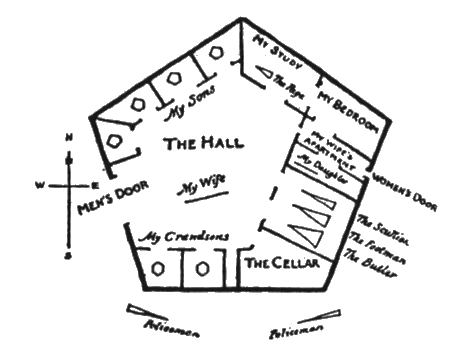
\includegraphics[trim=15mm 0mm 20mm 0mm,scale=0.5]{fig9}
\end{center}


I looked below, and saw with my physical eye all that domestic individuality
which I had hitherto merely inferred with the understanding. And how poor and
shadowy was the inferred conjecture in comparison with the reality which I now
behold! My four Sons calmly asleep in the North-Western rooms, my two orphan
Grandsons to the South; the Servants, the Butler, my Daughter, all in their
several apartments. Only my affectionate Wife, alarmed by my continued
absence, had quitted her room and was roving up and down in the Hall,
anxiously awaiting my return. Also the Page, aroused by my cries, had left his
room, and under pretext of ascertaining whether I had fallen somewhere in a
faint, was prying into the cabinet in my study. All this I could now \emph{see}, not
merely infer; and as we came nearer and nearer, I could discern even the
contents of my cabinet, and the two chests of gold, and the tablets of which
the Sphere had made mention.

Touched by my Wife's distress, I would have sprung downward to reassure her,
but I found myself incapable of motion. ``Trouble not yourself about your
Wife,'' said my Guide: ``she will not be long left in anxiety; meantime, let us
take a survey of Flatland.''

Once more I felt myself rising through space. It was even as the Sphere had
said. The further we receded from the object we beheld, the larger became the
field of vision. My native city, with the interior of every house and every
creature therein, lay open to my view in miniature. We mounted higher, and lo,
the secrets of the earth, the depths of the mines and inmost caverns of the
hills, were bared before me.

Awestruck at the sight of the mysteries of the earth, thus unveiled before my
unworthy eye, I said to my Companion, ``Behold, I am become as a God. For the
wise men in our country say that to see all things, or as they express it,
\emph{omnividence}, is the attribute of God alone.'' There was something of scorn in
the voice of my Teacher as he made answer: ``it is so indeed? Then the very
pick-pockets and cut-throats of my country are to be worshipped by your wise
men as being Gods: for there is not one of them that does not see as much as
you see now. But trust me, your wise men are wrong.''

\emph{I}. Then is omnividence the attribute of
others besides Gods?

\emph{SPHERE}. I do not know. But, if a pick-pocket or a cut-throat of our country
can see everything that is in your country, surely that is no reason why the
pick-pocket or cut-throat should be accepted by you as a God. This
omnividence, as you call it --- it is not a common word in Spaceland --- does it
make you more just, more merciful, less selfish, more loving? Not in the
least. Then how does it make you more divine?

\emph{I}. ``More merciful, more loving!'' But these are the qualities of women! And we
know that a Circle is a higher Being than a Straight Line, in so far as
knowledge and wisdom are more to be esteemed than mere affection.

\emph{SPHERE}. It is not for me to classify human faculties according to merit. Yet
many of the best and wisest in Spaceland think more of the affections than of
the understanding, more of your despised Straight Lines than of your belauded
Circles. But enough of this. Look yonder. Do you know that building?

I looked, and afar off I saw an immense Polygonal structure, in which I
recognized the General Assembly Hall of the States of Flatland, surrounded by
dense lines of Pentagonal buildings at right angles to each other, which I
knew to be streets; and I perceived that I was approaching the great
Metropolis.

``Here we descend,'' said my Guide. It was now morning, the first hour of the
first day of the two thousandth year of our era. Acting, as was their wont, in
strict accordance with precedent, the highest Circles of the realm were
meeting in solemn conclave, as they had met on the first hour of the first day
of the year 1000, and also on the first hour of the first day of the year 0.

The minutes of the previous meetings were now read by one whom I at once
recognized as my brother, a perfectly Symmetrical Square, and the Chief Clerk
of the High Council. It was found recorded on each occasion that: ``Whereas the
States had been troubled by divers ill-intentioned persons pretending to have
received revelations from another World, and professing to produce
demonstrations whereby they had instigated to frenzy both themselves and
others, it had been for this cause unanimously resolved by the Grand Council
that on the first day of each millenary, special injunctions be sent to the
Prefects in the several districts of Flatland, to make strict search for such
misguided persons, and without formality of mathematical examination, to
destroy all such as were Isosceles of any degree, to scourge and imprison any
regular Triangle, to cause any Square or Pentagon to be sent to the district
Asylum, and to arrest any one of higher rank, sending him straightway to the
Capital to be examined and judged by the Council.''

``You hear your fate,'' said the Sphere to me, while the Council was passing for
the third time the formal resolution. ``Death or imprisonment awaits the
Apostle of the Gospel of Three Dimensions.'' ``Not so,'' replied I, ``the matter
is now so clear to me, the nature of real space so palpable, that methinks I
could make a child understand it. Permit me but to descend at this moment and
enlighten them.'' ``Not yet,'' said my Guide, ``the time will come for that.
Meantime I must perform my mission. Stay thou there in thy place.'' Saying
these words, he leaped with great dexterity into the sea (if I may so call it)
of Flatland, right in the midst of the ring of Counsellors. ``I come,'' said he,
``to proclaim that there is a land of Three Dimensions.''

I could see many of the younger Counsellors start back in manifest horror, as
the Sphere's circular section widened before them. But on a sign from the
presiding Circle --- who shewed not the slightest alarm or surprise --- six
Isosceles of a low type from six different quarters rushed upon the Sphere.
``We have him,'' they cried; ``No; yes; we have him still! he's going! he's
gone!''

``My Lords,'' said the President to the Junior Circles of the Council, ``there is
not the slightest need for surprise; the secret archives, to which I alone
have access, tell me that a similar occurrence happened on the last two
millennial commencements. You will, of course, say nothing of these trifles
outside the Cabinet.''

Raising his voice, he now summoned the guards. ``Arrest the policemen; gag
them. You know your duty.'' After he had consigned to their fate the wretched
policemen --- ill-fated and unwilling witnesses of a State-secret which they
were not to be permitted to reveal --- he again addressed the Counsellors. ``My
Lords, the business of the Council being concluded, I have only to wish you a
happy New Year.'' Before departing, he expressed, at some length, to the Clerk,
my excellent but most unfortunate brother, his sincere regret that, in
accordance with precedent and for the sake of secrecy, he must condemn him to
perpetual imprisonment, but added his satisfaction that, unless some mention
were made by him of that day's incident, his life would be spared.


\chapter{How, though the Sphere showed me other mysteries of Spaceland, I still desire more; and what came of it} 


When I saw my poor brother led away to imprisonment, I attempted to leap down
into the Council Chamber, desiring to intercede on his behalf, or at least bid
him farewell. But I found that I had no motion of my own. I absolutely
depended on the volition of my Guide, who said in gloomy tones, ``Heed not thy
brother; haply thou shalt have ample time hereafter to condole with him.
Follow me.'' 
\begin{center}
    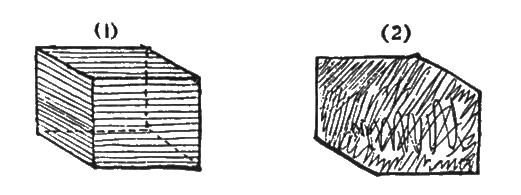
\includegraphics[trim=20mm 0mm 20mm 0mm,scale=0.5]{fig10}
\end{center}

Once more we ascended into space. ``Hitherto,'' said the Sphere, ``I have shewn
you naught save Plane Figures and their interiors. Now I must introduce you to
Solids, and reveal to you the plan upon which they are constructed. Behold
this multitude of moveable square cards. See, I put one on another, not, as
you supposed, Northward of the other, but \emph{on} the other. Now a second, now a
third. See, I am building up a Solid by a multitude of Squares parallel to one
another. Now the Solid is complete, being as high as it is long and broad, and
we call it a Cube.''

``Pardon me, my Lord,'' replied I; ``but to my eye the appearance is as of an
Irregular Figure whose inside is laid open to view; in other words, methinks I
see no Solid, but a Plane such as we infer in Flatland; only of an
Irregularity which betokens some monstrous criminal, so that the very sight of
it is painful to my eyes.''

``True,'' said the Sphere; ``it appears to you a Plane, because you are not
accustomed to light and shade and perspective; just as in Flatland a Hexagon
would appear a Straight Line to one who has not the Art of Sight Recognition.
But in reality it is a Solid, as you shall learn by the sense of Feeling.''

He then introduced me to the Cube, and I found that this marvellous Being was
indeed no Plane, but a Solid; and that he was endowed with six plane sides and
eight terminal points called solid angles; and I remembered the saying of the
Sphere that just such a Creature as this would be formed by the Square moving,
in Space, parallel to himself: and I rejoiced to think that so insignificant a
Creature as I could in some sense be called the Progenitor of so illustrious
an offspring.

But still I could not fully understand the meaning of what my Teacher had told
me concerning ``light'' and ``shade'' and ``perspective''; and I did not hesitate to
put my difficulties before him.

Were I to give the Sphere's explanation of these matters, succinct and clear
though it was, it would be tedious to an inhabitant of Space, who knows these
things already. Suffice it, that by his lucid statements, and by changing the
position of objects and lights, and by allowing me to feel the several objects
and even his own sacred Person, he at last made all things clear to me, so
that I could now readily distinguish between a Circle and a Sphere, a Plane
Figure and a Solid.

This was the Climax, the Paradise, of my strange eventful History. Henceforth
I have to relate the story of my miserable Fall: --- most miserable, yet surely
most undeserved! For why should the thirst for knowledge be aroused, only to
be disappointed and punished? My volition shrinks from the painful task of
recalling my humiliation; yet, like a second Prometheus, I will endure this
and worse, if by any means I may arouse in the interiors of Plane and Solid
Humanity a spirit of rebellion against the Conceit which would limit our
Dimensions to Two or Three or any number short of Infinity. Away then with all
personal considerations! Let me continue to the end, as I began, without
further digressions or anticipations, pursuing the plain path of dispassionate
History. The exact facts, the exact words, --- and they are burnt in upon my
brain, --- shall be set down without alteration of an iota; and let my Readers
judge between me and Destiny.

The Sphere would willingly have continued his lessons by indoctrinating me in
the conformation of all regular Solids, Cylinders, Cones, Pyramids,
Pentahedrons, Hexahedrons, Dodecahedrons, and Spheres: but I ventured to
interrupt him. Not that I was wearied of knowledge.  On the contrary, I
thirsted for yet deeper and fuller draughts than he was offering to me.

``Pardon me,'' said I, ``O Thou Whom I must no longer address as the Perfection
of all Beauty; but let me beg thee to vouchsafe thy servant a sight of thine
interior.''

\emph{SPHERE}. My what?

\emph{I}. Thine interior: thy stomach, thy intestines.

\emph{SPHERE}. Whence this ill-timed impertinent request? And what mean you by saying
that I am no longer the Perfection of all Beauty?

\emph{I}. My Lord, your own wisdom has taught me to aspire to One even more great,
more beautiful, and more closely approximate to Perfection than yourself. As
you yourself, superior to all Flatland forms, combine many Circles in One, so
doubtless there is One above you who combines many Spheres in One Supreme
Existence, surpassing even the Solids of Spaceland. And even as we, who are
now in Space, look down on Flatland and see the insides of all things, so of a
certainty there is yet above us some higher, purer region, whither thou dost
surely purpose to lead me --- O Thou Whom I shall always call, everywhere and in
all Dimensions, my Priest, Philosopher, and Friend --- some yet more spacious
Space, some more dimensionable Dimensionality, from the vantage-ground of
which we shall look down together upon the revealed insides of Solid things,
and where thine own intestines, and those of thy kindred Spheres, will lie
exposed to the view of the poor wandering exile from Flatland, to whom so much
has already been vouchsafed.

\emph{SPHERE}. Pooh! Stuff! Enough of this trifling! The time is short, and much
remains to be done before you are fit to proclaim the Gospel of Three
Dimensions to your blind benighted countrymen in Flatland.

\emph{I}. Nay, gracious Teacher, deny me not what I know it is in thy power to
perform. Grant me but one glimpse of thine interior, and I am satisfied for
ever, remaining henceforth thy docile pupil, thy unemancipable slave, ready to
receive all thy teachings and to feed upon the words that fall from thy lips.

\emph{SPHERE}. Well, then, to content and silence you, let me say at once, I would
shew you what you wish if I could; but I cannot. Would you have me turn my
stomach inside out to oblige you?

\emph{I}. But my Lord has shewn me the intestines of all my countrymen in the Land of
Two Dimensions by taking me with him into the Land of Three. What therefore
more easy than now to take his servant on a second journey into the blessed
region of the Fourth Dimension, where I shall look down with him once more
upon this land of Three Dimensions, and see the inside of every
three-dimensioned house, the secrets of the solid earth, the treasures of the
mines of Spaceland, and the intestines of every solid living creature, even
the noble and adorable Spheres.

\emph{SPHERE}. But where is this land of Four Dimensions?

\emph{I}. I know not: but doubtless my Teacher knows.

\emph{SPHERE}. Not I. There is no such land. The very idea of it is utterly
inconceivable.

\emph{I}. Not inconceivable, my Lord, to me, and therefore still less inconceivable
to my Master. Nay, I despair not that, even here, in this region of Three
Dimensions, your Lordship's art may make the Fourth Dimension visible to me;
just as in the Land of Two Dimensions my Teacher's skill would fain have
opened the eyes of his blind servant to the invisible presence of a Third
Dimension, though I saw it not.

Let me recall the past. Was I not taught below that when I saw a Line and
inferred a Plane, I in reality saw a Third unrecognized Dimension, not the
same as brightness, called ``height''? And does it not now follow that, in this
region, when I see a Plane and infer a Solid, I really see a Fourth
unrecognized Dimension, not the same as colour, but existent, though
infinitesimal and incapable of measurement?

And besides this, there is the Argument from Analogy of Figures.

\emph{SPHERE}. Analogy! Nonsense: what analogy?

I. Your Lordship tempts his servant to see whether he remembers the
revelations imparted to him. Trifle not with me, my Lord; I crave, I thirst,
for more knowledge. Doubtless we cannot \emph{see} that other higher Spaceland now,
because we have no eye in our stomachs. But, just as there \emph{was} the realm of
Flatland, though that poor puny Lineland Monarch could neither turn to left
nor right to discern it, and just as there \emph{was} close at hand, and touching my
frame, the land of Three Dimensions, though I, blind senseless wretch, had no
power to touch it, no eye in my interior to discern it, so of a surety there
is a Fourth Dimension, which my Lord perceives with the inner eye of thought.
And that it must exist my Lord himself has taught me. Or can he have forgotten
what he himself imparted to his servant?

In One Dimension, did not a moving Point produce a Line with \emph{two} terminal
points?

In Two Dimensions, did not a moving Line produce a Square with \emph{four} terminal
points?

In Three Dimensions, did not a moving Square produce --- did not this eye of
mine behold it --- that blessed Being, a Cube, with \emph{eight} terminal points?

And in Four Dimensions shall not a moving Cube --- alas, for Analogy, and alas
for the Progress of Truth, if it be not so --- shall not, I say, the motion of a
divine Cube result in a still more divine Organization with \emph{sixteen} terminal
points?

Behold the infallible confirmation of the Series, 2, 4,
8, 16: is not this a Geometrical Progression? Is not this --- if I might quote
my Lord's own words --- ``strictly according to Analogy''?

Again, was I not taught by my Lord that as in a Line there are \emph{two} bounding
Points, and in a Square there are \emph{four} bounding Lines, so in a Cube there must
be \emph{six} bounding Squares? Behold once more the confirming Series, 2, 4, 6: is
not this an Arithmetical Progression? And consequently does it not of
necessity follow that the more divine offspring of the divine Cube in the Land
of Four Dimensions, must have 8 bounding Cubes: and is not this also, as my
Lord has taught me to believe, ``strictly according to Analogy''?

O, my Lord, my Lord, behold, I cast myself in faith upon conjecture, not
knowing the facts; and I appeal to your Lordship to confirm or deny my logical
anticipations. If I am wrong, I yield, and will no longer demand a Fourth
Dimension; but, if I am right, my Lord will listen to reason.

I ask therefore, is it, or is it not, the fact, that ere now your countrymen
also have witnessed the descent of Beings of a higher order than their own,
entering closed rooms, even as your Lordship entered mine, without the opening
of doors or windows, and appearing and vanishing at will? On the reply to this
question I am ready to stake everything. Deny it, and I am henceforth silent.
Only vouchsafe an answer.

\emph{SPHERE} (\emph{after a pause}). It is reported so. But men are divided in opinion as
to the facts. And even granting the facts, they explain them in different
ways. And in any case, however great may be the number of different
explanations, no one has adopted or suggested the theory of a Fourth
Dimension. Therefore, pray have done with this trifling, and let us return to
business.

\emph{I}. I was certain of it. I was certain that my anticipations would be
fulfilled. And now have patience with me and answer me yet one more question,
best of Teachers! Those who have thus appeared --- no one knows whence --- and
have returned --- no one knows whither --- have they also contracted their
sections and vanished somehow into that more Spacious Space, whither I now
entreat you to conduct me?

\emph{SPHERE} (\emph{moodily}). They have vanished, certainly --- if they ever appeared. But
most people say that these visions arose from the thought --- you will not
understand me --- from the brain; from the perturbed angularity of the Seer.

I. Say they so? Oh, believe them not. Or if it indeed be so, that this other
Space is really Thoughtland, then take me to that blessed Region where I in
Thought shall see the insides of all solid things. There, before my ravished
eye, a Cube moving in some altogether new direction, but strictly according to
Analogy, so as to make every particle of his interior pass through a new kind
of Space, with a wake of its own --- shall create a still more perfect
perfection than himself, with sixteen terminal Extra-solid angles, and Eight
solid Cubes for his Perimeter. And once there, shall we stay our upward
course? In that blessed region of Four Dimensions, shall we linger at the
threshold of the Fifth, and not enter therein? Ah, no! Let us rather resolve
that our ambition shall soar with our corporal ascent. Then, yielding to our
intellectual onset, the gates of the Six Dimension shall fly open; after that
a Seventh, and then an Eighth ---

How long I should have continued I know not.  In vain did the Sphere, in his
voice of thunder, reiterate his command of silence, and threaten me with the
direst penalties if I persisted. Nothing could stem the flood of my ecstatic
aspirations. Perhaps I was to blame; but indeed I was intoxicated with the
recent draughts of Truth to which he himself had introduced me. However, the
end was not long in coming. My words were cut short by a crash outside, and a
simultaneous crash inside me, which impelled me through space with a velocity
that precluded speech. Down! down! down! I was rapidly descending; and I knew
that return to Flatland was my doom. One glimpse, one last and
never-to-be-forgotten glimpse I had of that dull level wilderness --- which was
now to become my Universe again --- spread out before my eye. Then a darkness.
Then a final, all-consummating thunder-peal; and, when I came to myself, I was
once more a common creeping Square, in my Study at home, listening to the
Peace-Cry of my approaching Wife.


\chapter{How the Sphere encouraged me in a Vision}


Although I had less than a minute for reflection, I felt, by a kind of
instinct, that I must conceal my experiences from my Wife. Not that I
apprehended, at the moment, any danger from her divulging my secret, but I
knew that to any Woman in Flatland the narrative of my adventures must needs
be unintelligible. So I endeavoured to reassure her by some story, invented
for the occasion, that I had accidentally fallen through the trap-door of the
cellar, and had there lain stunned.

The Southward attraction in our country is so slight that even to a Woman my
tale necessarily appeared extraordinary and well-nigh incredible; but my Wife,
whose good sense far exceeds that of the average of her Sex, and who perceived
that I was unusually excited, did not argue with me on the subject, but
insisted that I was ill and required repose. I was glad of an excuse for
retiring to my chamber to think quietly over what had happened. When I was at
last by myself, a drowsy sensation fell on me; but before my eyes closed I
endeavoured to reproduce the Third Dimension, and especially the process by
which a Cube is constructed through the motion of a Square. It was not so
clear as I could have wished; but I remembered that it must be ``Upward, and
yet not Northward,'' and I determined steadfastly to retain these words as the
clue which, if firmly grasped, could not fail to guide me to the solution. So
mechanically repeating, like a charm, the words, ``Upward, yet not Northward,''
I fell into a sound refreshing sleep.

During my slumber I had a dream. I thought I was once more by the side of the
Sphere, whose lustrous hue betokened that he had exchanged his wrath against
me for perfectly placability. We were moving together towards a bright but
infinitesimally small Point, to which my Master directed my attention. As we
approached, methought there issued from it a slight humming noise as from one
of your Spaceland bluebottles, only less resonant by far, so slight indeed
that even in the perfect stillness of the Vacuum through which we soared, the
sound reached not our ears till we checked our flight at a distant from it of
something under twenty human diagonals.

``Look yonder,'' said my Guide, ``in Flatland thou hast lived; of Lineland thou
hast received a vision; thou hast soared with me to the heights of Spaceland;
now, in order to complete the range of thy experience, I conduct thee downward
to the lowest depth of existence, even to the realm of Pointland, the Abyss of
No dimensions.

``Behold yon miserable creature. That Point is a Being like ourselves, but
confined to the non-dimensional Gulf. He is himself his own World, his own
Universe; of any other than himself he can form no conception; he knows not
Length, nor Breadth, nor Height, for he has had no experience of them; he has
no cognizance even of the number Two; nor has he a thought of Plurality; for
he is himself his One and All, being really Nothing. Yet mark his perfect
self-contentment, and hence learn his lesson, that to be self-contented is to
be vile and ignorant, and that to aspire is better than to be blindly and
impotently happy. Now listen.''

He ceased; and there arose from the little buzzing creature a tiny, low,
monotonous, but distinct tinkling, as from one of your Spaceland phonographs,
from which I caught these words, ``Infinite beatitude of existence! It is; and
there is nothing else beside It.''

``What,'' said I, ``does the puny creature mean by `it'?'' ``He means himself,''
said the Sphere: ``have you not noticed before now, that babies and babyish
people who cannot distinguish themselves from the world, speak of themselves
in the Third Person? But hush!''

``It fills all Space,'' continued the little soliloquizing Creature, ``and what
It fills, It is. What It thinks, that It utters; and what It utters, that It
hears; and It itself is Thinker, Utterer, Hearer, Thought, Word, Audition; it
is the One, and yet the All in All. Ah, the happiness, ah, the happiness of
Being!''

``Can you not startle the little thing out of its complacency?'' said I. ``Tell
it what it really is, as you told me; reveal to it the narrow limitations of
Pointland, and lead it up to something higher.'' ``That is no easy task,'' said
my Master; ``try you.''

Hereon, raising by voice to the uttermost, I addressed the Point as follows:

``Silence, silence, contemptible Creature. You call yourself the All in All,
but you are the Nothing: your so-called Universe is a mere speck in a Line,
and a Line is a mere shadow as compared with ---'' ``Hush, hush, you have said
enough,'' interrupted the Sphere, ``now listen, and mark the effect of your
harangue on the King of Pointland.''

The lustre of the Monarch, who beamed more brightly than ever upon hearing my
words, shewed clearly that he retained his complacency; and I had hardly
ceased when he took up his strain again. ``Ah, the joy, ah, the joy of Thought!
What can It not achieve by thinking! Its own Thought coming to Itself,
suggestive of its disparagement, thereby to enhance Its happiness! Sweet
rebellion stirred up to result in triumph! Ah, the divine creative power of
the All in One! Ah, the joy, the joy of Being!''

``You see,'' said my Teacher, ``how little your words have done. So far as the
Monarch understand them at all, he accepts them as his own --- for he cannot
conceive of any other except himself --- and plumes himself upon the variety of
`Its Thought' as an instance of creative Power. Let us leave this God of
Pointland to the ignorant fruition of his omnipresence and omniscience:
nothing that you or I can do can rescue him from his self-satisfaction.''

After this, as we floated gently back to Flatland, I could hear the mild voice
of my Companion pointing the moral of my vision, and stimulating me to aspire,
and to teach others to aspire. He had been angered at first --- he confessed ---
by my ambition to soar to Dimensions above the Third; but, since then, he had
received fresh insight, and he was not too proud to acknowledge his error to a
Pupil. Then he proceeded to initiate me into mysteries yet higher than those I
had witnessed, shewing me how to construct Extra-Solids by the motion of
Solids, and Double Extra-Solids by the motion of Extra-Solids, and all
``strictly according to Analogy,'' all by methods so simple, so easy, as to be
patent even to the Female Sex.?


\chapter{How I tried to teach the Theory of Three Dimensions to my Grandson, and with what success}


I awoke rejoicing, and began to reflect on the glorious career before me. I
would go forth, methought, at once, and evangelize the whole of Flatland. Even
to Women and Soldiers should the Gospel of Three Dimensions be proclaimed. I
would begin with my Wife.

Just as I had decided on the plan of my operations, I heard the sound of many
voices in the street commanding silence. Then followed a louder voice. It was
a herald's proclamation. Listening attentively, I recognized the words of the
Resolution of the Council, enjoining the arrest, imprisonment, or execution of
any one who should pervert the minds of people by delusions, and by professing
to have received revelations from another World.

I reflected. This danger was not to be trifled with. It would be better to
avoid it by omitting all mention of my Revelation, and by proceeding on the
path of Demonstration --- which after all, seemed so simple and so conclusive
that nothing would be lost by discarding the former means. ``Upward, not
Northward'' --- was the clue to the whole proof. It had seemed to me fairly clear
before I fell asleep; and when I first awoke, fresh from my dream, it had
appeared as patent as Arithmetic; but somehow it did not seem to me quite so
obvious now. Though my Wife entered the room opportunely at just that moment,
I decided, after we had exchanged a few words of commonplace conversation, not
to begin with her.

My Pentagonal Sons were men of character and standing, and physicians of no
mean reputation, but not great in mathematics, and, in that respect, unfit for
my purpose. But it occurred to me that a young and docile Hexagon, with a
mathematical turn, would be a most suitable pupil. Why therefore not make my
first experiment with my little precocious Grandson, whose casual remarks on
the meaning of three-to-the-third had met with the approval of the Sphere?
Discussing the matter with him, a mere boy, I should be in perfect safety; for
he would know nothing of the Proclamation of the Council; whereas I could not
feel sure that my Sons --- so greatly did their patriotism and reverence for the
Circles predominate over mere blind affection --- might not feel compelled to
hand me over to the Prefect, if they found me seriously maintaining the
seditious heresy of the Third Dimension.

But the first thing to be done was to satisfy in some way the curiosity of my
Wife, who naturally wished to know something of the reasons for which the
Circle had desired that mysterious interview, and of the means by which he had
entered the house. Without entering into the details of the elaborate account
I gave her, --- an account, I fear, not quite so consistent with truth as my
Readers in Spaceland might desire, --- I must be content with saying that I
succeeded at last in persuading her to return quietly to her household duties
without eliciting from me any reference to the World of Three Dimensions. This
done, I immediately sent for my Grandson; for, to confess the truth, I felt
that all that I had seen and heard was in some strange way slipping away from
me, like the image of a half- grasped, tantalizing dream, and I longed to
essay my skill in making a first disciple.

When my Grandson entered the room I carefully secured the door. Then, sitting
down by his side and taking our mathematical tablets, --- or, as you would call
them, Lines --- I told him we would resume the lesson of yesterday. I taught him
once more how a Point by motion in One Dimension produces a Line, and how a
straight Line in Two Dimensions produces a Square. After this, forcing a
laugh, I said, ``And now, you scamp, you wanted to make believe that a Square
may in the same way by motion `Upward, not Northward' produce another figure,
a sort of extra square in Three Dimensions. Say that again, you young rascal.''

At this moment we heard once more the herald's ``O yes! O yes!'' outside in the
street proclaiming the Resolution of the Council. Young though he was, my
Grandson --- who was unusually intelligent for his age, and bred up in perfect
reverence for the authority of the Circles --- took in the situation with an
acuteness for which I was quite unprepared. He remained silent till the last
words of the Proclamation had died away, and then, bursting into tears, ``Dear
Grandpapa,'' he said, ``that was only my fun, and of course I meant nothing at
all by it; and we did not know anything then about the new Law; and I don't
think I said anything about the Third Dimension; and I am sure I did not say
one word about `Upward, not Northward,' for that would be such nonsense, you
know. How could a thing move Upward, and not Northward? Upward and not
Northward! Even if I were a baby, I could not be so absurd as that. How silly
it is! Ha! ha! ha!''

``Not at all silly,'' said I, losing my temper; ``here for example, I take this
Square,'' and, at the word, I grasped a moveable Square, which was lying at
hand --- ``and I move it, you see, not Northward but --- yes, I move it Upward ---
that is to say, Northward but I move it somewhere --- not exactly like this, but
somehow ---'' Here I brought my sentence to an inane conclusion, shaking the
Square about in a purposeless manner, much to the amusement of my Grandson,
who burst out laughing louder than ever, and declared that I was not teaching
him, but joking with him; and so saying he unlocked the door and ran out of
the room. Thus ended my first attempt to convert a pupil to the Gospel of
Three Dimensions.


\chapter{How I then tried to diffuse the Theory of Three Dimensions by other means, and of the result} 


My failure with my Grandson did not encourage me to communicate my secret to
others of my household; yet neither was I led by it to despair of success.
Only I saw that I must not wholly rely on the catch-phrase, ``Upward, not
Northward,'' but must rather endeavour to seek a demonstration by setting
before the public a clear view of the whole subject; and for this purpose it
seemed necessary to resort to writing.

So I devoted several months in privacy to the composition of a treatise on the
mysteries of Three Dimensions. Only, with the view of evading the Law, if
possible, I spoke not of a physical Dimension, but of a Thoughtland whence, in
theory, a Figure could look down upon Flatland and see simultaneously the
insides of all things, and where it was possible that there might be supposed
to exist a Figure environed, as it were, with six Squares, and containing
eight terminal Points. But in writing this book I found myself sadly hampered
by the impossibility of drawing such diagrams as were necessary for my
purpose: for of course, in our country of Flatland, there are no tablets but
Lines, and no diagrams but Lines, all in one straight Line and only
distinguishable by difference of size and brightness; so that, when I had
finished my treatise (which I entitled, ``Through Flatland to Thoughtland'') I
could not feel certain that many would understand my meaning.

Meanwhile my life was under a cloud. All pleasures palled upon me; all sights
tantalized and tempted me to outspoken treason, because I could not but
compare what I saw in Two Dimensions with what it really was if seen in Three,
and could hardly refrain from making my comparisons aloud. I neglected my
clients and my own business to give myself to the contemplation of the
mysteries which I had once beheld, yet which I could impart to no one, and
found daily more difficult to reproduce even before my own mental vision.

One day, about eleven months after my return from Spaceland, I tried to see a
Cube with my eye closed, but failed; and though I succeeded afterwards, I was
not then quite certain (nor have I been ever afterwards) that I had exactly
realized the original. This made me more melancholy than before, and
determined me to take some step; yet what, I knew not. I felt that I would
have been willing to sacrifice my life for the Cause, if thereby I could have
produced conviction. But if I could not convince my Grandson, how could I
convince the highest and most developed Circles in the land?

And yet at times my spirit was too strong for me, and I gave vent to
dangerous utterances. Already I was considered heterodox if not treasonable,
and I was keenly alive to the danger of my position; nevertheless I could not
at times refrain from bursting out into suspicious or half-seditious
utterances, even among the highest Polygonal or Circular society. When, for
example, the question arose about the treatment of those lunatics who said
that they had received the power of seeing the insides of things, I would
quote the saying of an ancient Circle, who declared that prophets and inspired
people are always considered by the majority to be mad; and I could not help
occasionally dropping such expressions as ``the eye that discerns the interiors
of things,'' and ``the all-seeing land''; once or twice I even let fall the
forbidden terms ``the Third and Fourth Dimensions.'' At last, to complete a
series of minor indiscretions, at a meeting of our Local Speculative Society
held at the palace of the Prefect himself, --- some extremely silly person
having read an elaborate paper exhibiting the precise reasons why Providence
has limited the number of Dimensions to Two, and why the attribute of
omnividence is assigned to the Supreme alone --- I so far forgot myself as to
give an exact account of the whole of my voyage with the Sphere into Space,
and to the Assembly Hall in our Metropolis, and then to Space again, and of my
return home, and of everything that I had seen and heard in fact or vision. At
first, indeed, I pretended that I was describing the imaginary experiences of
a fictitious person; but my enthusiasm soon forced me to throw off all
disguise, and finally, in a fervent peroration, I exhorted all my hearers to
divest themselves of prejudice and to become believers in the Third Dimension.

Need I say that I was at once arrested and taken before the Council?

Next morning, standing in the very place where but a very few months ago the
Sphere had stood in my company, I was allowed to begin and to continue my
narration unquestioned and uninterrupted. But from the first I foresaw my
fate; for the President, noting that a guard of the better sort of Policemen
was in attendance, of angularity little, if at all, under 55 degrees, ordered
them to be relieved before I began my defence, by an inferior class of 2 or 3
degrees. I knew only too well what that meant. I was to be executed or
imprisoned, and my story was to be kept secret from the world by the
simultaneous destruction of the officials who had heard it; and, this being
the case, the President desired to substitute the cheaper for the more
expensive victims.

After I had concluded my defence, the President, perhaps perceiving that some
of the junior Circles had been moved by evident earnestness, asked me two
questions: ---

\begin{enumerate}
    \item Whether I could indicate the direction which I meant when I used the
          words ``Upward, not Northward''?  
    \item Whether I could by any diagrams or descriptions (other than the
          enumeration of imaginary sides and angles) indicate the Figure I was
          pleased to call a Cube?  I declared that I could say nothing more, and
          that I must commit myself to the Truth, whose cause would surely
          prevail in the end.
\end{enumerate}

The President replied that he quite concurred in my sentiment, and that I
could not do better. I must be sentenced to perpetual imprisonment; but if the
Truth intended that I should emerge from prison and evangelize the world, the
Truth might be trusted to bring that result to pass. Meanwhile I should be
subjected to no discomfort that was not necessary to preclude escape, and,
unless I forfeited the privilege by misconduct, I should be occasionally
permitted to see my brother who had preceded me to my prison.

Seven years have elapsed and I am still a prisoner, and --- if I except the
occasional visits of my brother --- debarred from all companionship save that of
my jailers. My brother is one of the best of Squares, just sensible, cheerful,
and not without fraternal affection; yet I confess that my weekly interviews,
at least in one respect, cause me the bitterest pain. He was present when the
Sphere manifested himself in the Council Chamber; he saw the Sphere's changing
sections; he heard the explanation of the phenomena then give to the Circles.
Since that time, scarcely a week has passed during seven whole years, without
his hearing from me a repetition of the part I played in that manifestation,
together with ample descriptions of all the phenomena in Spaceland, and the
arguments for the existence of Solid things derivable from Analogy. Yet --- I
take shame to be forced to confess it --- my brother has not yet grasped the
nature of Three Dimensions, and frankly avows his disbelief in the existence
of a Sphere.

Hence I am absolutely destitute of converts, and, for
aught that I can see, the millennial Revelation has been made to me for
nothing. Prometheus up in Spaceland was bound for bringing down fire for
mortals, but I --- poor Flatland Prometheus --- lie here in prison for bringing
down nothing to my countrymen. Yet I exist in the hope that these memoirs, in
some manner, I know not how, may find their way to the minds of humanity in
Some Dimension, and may stir up a race of rebels who shall refuse to be
confined to limited Dimensionality.

That is the hope of my brighter moments. Alas, it is
not always so. Heavily weights on me at times the burdensome reflection that I
cannot honestly say I am confident as to the exact shape of the once-seen,
oft-regretted Cube; and in my nightly visions the mysterious precept, ``Upward,
not Northward,'' haunts me like a soul-devouring Sphinx. It is part of the
martyrdom which I endure for the cause of Truth that there are seasons of
mental weakness, when Cubes and Spheres flit away into the background of
scarce-possible existences; when the Land of Three Dimensions seems almost as
visionary as the Land of One or None; nay, when even this hard wall that bars
me from my freedom, these very tablets on which I am writing, and all the
substantial realities of Flatland itself, appear no better than the offspring
of a diseased imagination, or the baseless fabric of a dream.
\begin{center}
    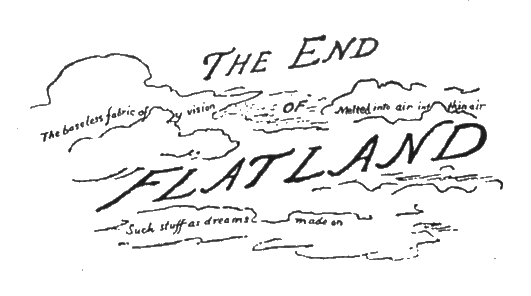
\includegraphics[trim=20mm 0mm 0mm 0mm, scale=0.4]{fig11}
\end{center}

\end{document}

